\documentclass[landscape,a4paper]{amsart}

\usepackage{amsthm, amsmath, amsfonts}
\usepackage{amssymb,latexsym}
\usepackage[alphabetic]{amsrefs}
\usepackage[mathscr]{eucal}
\usepackage{pdfsync}
\usepackage{graphicx}
\usepackage{epstopdf}
\DeclareGraphicsRule{.tif}{png}{.png}{`convert #1 `dirname #1`/`basename #1 .tif`.png}
\usepackage[all]{xy}
\usepackage{titletoc}

\CompileMatrices

\theoremstyle{plain}
\newtheorem{theorem}{Theorem}[section]
\newtheorem{lemma}[theorem]{Lemma}
\newtheorem{proposition}[theorem]{Proposition}
\newtheorem{corollary}[theorem]{Corollary}

\theoremstyle{definition}
\newtheorem{definition}[theorem]{Definition}%[section]

\theoremstyle{remark}
\newtheorem{example}[theorem]{Example}
\newtheorem{remark}[theorem]{Remark}
\newtheorem{discussion}[theorem]{Discussion}

%\numberwithin{equation}{section}

%\newcommand{\abs}[1]{\lvert#1\rvert}

%\newcommand{\blankbox}[2]{%
%  \parbox{\columnwidth}{\centering
%%    Set fboxsep to 0 so that the actual size of the box will match the
%%    given measurements more closely.
%    \setlength{\fboxsep}{0pt}%
%    \fbox{\raisebox{0pt}[#2]{\hspace{#1}}}%
%  }%
%}

\DeclareMathOperator{\Lip}{Lip}
\DeclareMathOperator{\dist}{dist}
\DeclareMathOperator{\expected}{\mathbb{E}}
\DeclareMathOperator{\prb}{Prob}
\DeclareMathOperator{\spt}{spt}
\DeclareMathOperator{\lap}{\Delta}
\DeclareMathOperator{\Tr}{Tr}

\raggedbottom

\setlength{\textwidth}{25cm}
\setlength{\oddsidemargin}{-1cm}
\setlength{\evensidemargin}{-1cm}
\setlength{\textheight}{17cm}
%\addtolength{\oddsidemargin}{-1cm}
%\addtolength{\evensidemargin}{-1cm} 
%\addtolength{\topmargin}{-1cm} 
%\addtolength{\textheight}{2cm}
% \renewcommand{\l@subsection}{\@contentsline{2}{5em}{7em}}

%\makeatletter
%\makeatother

 
%%% BEGIN DOCUMENT
\begin{document}

\title{Graphs: Electric Current and Random Walk Interpretations}  
\author{John E.\ Hutchinson}
\date{\today}

%\begin{abstract} We build up the basics of finite graphs and their interpretations via electric currents, random walks and   matrices, sufficient to develop analysis on fractals.
%\end{abstract}

%\maketitle


%\begin{table}[htdp]
%\caption{default}
\begin{center}

\begin{tabular}{p{5cm} p{5cm} p{5cm} p{5cm} p{5cm}}

&

 \hfill  \textbf{Analytic}  \hfill \mbox{}

&   \hfill  \textbf{Electric Network}  \hfill \mbox{}

&  \hfill   \textbf{Random Walk}  \hfill \mbox{}

&   \hfill  \textbf{Linear Algebra}  \hfill \mbox{}   % end of column heads
  
\\  \hline \\ \rule{0pt}{12pt} \\  \hfill \mbox{}

\textbf{Laplacian}  $ \lap f(x)   $ 

& \hfill $   \left(  \sum_{y\sim x}  \dfrac{c_{xy}}{c_x} f(y)\right) -  f(x) $  \hfill \mbox{} \newline
(difference between weighted average of $ f $ at neighbours of $ x $ and value of $ f $ at $ x $)

&  \hfill $  -\dfrac{i_x}{c_x} $ \hfill  \mbox{} \newline
  ($ f ( z ) $ is  voltage at $ z$,   \newline
    $ i_{x} =  \sum_y c_{xy} (f(x) - f(y)) $ is current out of $ x $)

&  \hfill $   \mathbb{E}^x f(X_1) - f(x) $  \hfill  \mbox{}  

&  \hfill $ \lap = D^{-1}A = -(I - P) $ \hfill \mbox{} \newline
($P $ is transition matrix, \newline
$D  $ is diagonal with $D_{xx} = c_x $,\newline
$ A   $  is  conductance matrix)% end of row one

 \\   \rule{0pt}{12pt} \\  \hline \\ \rule{0pt}{12pt} \\ 

\textbf{Dirichlet Problem}\newline
$ G $ is ``boundary'', \newline
$ H = V\setminus G$ is ``interior''

&  $ f=g $ on $ G $, $ \lap f = 0 $ on $ H $ \newline
(uniqueness and hence existence from max pple) 

& $ f $ gives  voltages on $ H $ for  applied voltages $ g $ on $ G $ 

& \hfill $ f(x) = \mathbb{E}^x g(X_{T_G}) $ \hfill \mbox{} 
\mbox{} \qquad ($ = P^x(T_a < T_b ) $ if $ G=\{a,b\} $)
 
&  \hfill $ f_H = - A_{HH}^{-1} A_{HG}\, g $ \hfill \mbox{}\newline  
where $ A = \begin{bmatrix} A_{GG} &A_{GH}\\ A_{HG} &A_{HH} \end{bmatrix} $ \newline 
(solve $  f_G = g $, \newline
$ D^{-1} A_{HG} f_G + D^{-1} A_{HH} f_H = 0 $)        % end of row 2

 \\   \rule{0pt}{12pt} \\  \hline \\ \rule{0pt}{12pt} \\ 

\textbf{Green's Function} $ \mathcal{G}^G_a $ \newline
 (for fixed $ G $ and $ a \in H=  G^c $)

& $ -\lap \mathcal{G}^G_a = \dfrac{1}{c_a} \mathcal{X}_a \text{ on } H $ \newline
 \mbox{} \quad\  $    \mathcal{G}^G_a = 0 \text{ on } G $ \newline
(uniqueness and hence existence from max pple) 

& $ \mathcal{G}^G_a $ is harmonic extension of voltage  at $ a $ and zero voltage at $ G $ s.t.\  \emph{unit current} flows from $ a $ to $ G $ 

& $  \mathcal{G}^G_a(x) = \dfrac{1}{c_x}\mathbb{E}^a V_{x\to G} $ \newline
 \mbox{} \qquad\  = $\dfrac{1}{c_{xz}}\mathbb{E} ^a \Tr_{xz\to G} \text{ if } z \sim x $ \newline
\mbox{} \qquad \ $ =   \mathbb{R}_{aG}   P^x (T_a < T_G) $ \newline
(verify  eqns for first  and  third except at $ a $, evaluate both at $ a $; second follows from first
with $ Tr_{{xz}\to G} $ the no of traverses of $ xz $ on way to   $ G$)

& \hfill $ \mathcal{G}^G_a |_H =- [ A_{HH}^{-1}]_a $, \hfill \mbox{}\newline
 where $  [M]_a$  is col $ a $ of matrix $ M $\newline
 (solve $ (I_H - P_{HH})\mathcal{G}^G_a  =[D_H^{-1}]_a) $ 
% where $  [M]_a$  is col $ a $ of matrix $ M $) 

%$ \mathcal{G}^G_a |_H $ is col $ a $ of $ A_{HH}^{-1} $ \hfill \mbox{}\newline
% (solve $ (I_H - P_{HH})\mathcal{G}^G_a  =[D_H^{-1}]_a $\newline
% where $  [M]_a$  is col $ a $ of matrix $ M $) 

 \\   \rule{0pt}{12pt} \\  \hline \\ \rule{0pt}{12pt} \\    % end of row 3
 
\textbf{Effective Resistance} $ \mathbb{R}_{aG} $  \newline
($ G = \{ b \} $ gives a \emph{metric} $ \mathbb{R}_{ab} $)

&  \hfill $ \mathbb{R}_{aG} = \mathcal{G}^G_a(a) $ \hfill \mbox{} \newline
(Green's function for bdy $ G $)
 
& \mbox{}\emph{Defn}: $ \mathbb{R}_{aG} := \mathcal{G}^G_a(a) $ is voltage at $ a $ s.t.\  zero voltage at $ G $ induces a unit flow from $ a $ to $ G $ 
 
 
& $  \mathbb{R}_{aG} = \dfrac{1}{c_a}\mathbb{E}^a V_{a\to G} $ \newline
\mbox{} \qquad \ $ =   \big( c_a P^a (T_G < T^+_a)\big)^{-1} $ \newline
(the first equality by defn, the second by standard prob thy)
 
 &   \hfill $   \mathbb{R}_{aG} = -(A_{HH}^{-1})_{aa} $ \hfill \mbox{}\newline


\end{tabular}
\end{center}
%\label{default}
%\end{table}%


\end{document} 




















%\renewcommand*\l@subsection{\@tocline{4}{50em}{7em}{10em}{10em}}

\tableofcontents




 

\section{\textbf{Graphs}}  \label{secint}

\begin{figure}[htbp] %  figure placement: here, top, bottom, or page
   \centering
   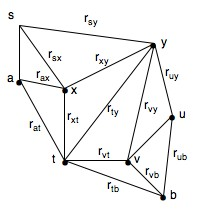
\includegraphics[width=2in]{graph.jpg} 
   \caption{A finite graph}
   \label{graph}
\end{figure}

A \emph{(finite) graph} is a triple
\[  G = (V,E, r_{xy} ) \]
where 
\begin{itemize}
\item $ V $ is the finite set of \emph{vertices} or \emph{nodes},
\item $ E $ is the set of \emph{edges} and consists of certain pairs of distinct vertices,
\item $ r_{xy} $ is a (strictly) \emph{positive} function defined on $ E $.
\end{itemize}
Note $ r_{xy} = r_{yx} $.

We assume the graph to be \emph{connected}.

\subsection{Notation and Definitions}
\begin{itemize}
\item Write $ x\sim y $ if $ \{x,y\} \in E $.
\item A \emph{simple} graph is one such that $ r_{xy} \equiv 1 $ for $ \{x,y\}\in E$.
\item  $ c_{xy} := 1/r_{xy}$.    

If $ xy $ is not an edge define $ c_{xy} = 0$.  

$r_{xy} $ is the \emph{resistance} of the edge $ xy$ and $ c_{xy} $ is the \emph{conductance}.

\item The \emph{weighted degree} of $ x $ is $ c_x := \sum_y c_{xy} $.
It is the number of edges from $ x $ if $ G $ is simple and in this case is just called the \emph{degree} of $ x $.

\item The \emph{total mass} of $ G $ is $ C = C(G) := \sum_x c_x $. \label{tm}  In the case of a simple graph it is twice the number of edges, or equivalently the sum of the degrees of the vertices.

\end{itemize} 


%%%%%%%%%%%%%%%%%%%%%%%%%%%%%%%%
%%%%%%%%%%%%%%%%%%%%%%%%%%%%%%%%
%%%%%%%%%%%%%%%%%%%%%%%%%%%%%%%%

\section{\textbf{Electric Network Interpretation of a Graph}}  \label{secEN}

Fix a graph $ G $ and fix \emph{boundary} vertices $ a \neq b $.  Other vertices are called \emph{interior}.  
(More generally, the boundary vertices are any nonempty set $ B = \partial V \subset V $ and the interior vertices are $ V^\circ = V \setminus \partial V $.  See Section~\ref{secfc}.)

\subsection{Physical Motivation} \label{pm} Think of $ G $ as an electric network [EN] with resistance $ r_{xy} $ on the edge $ xy $.
External voltages $ v(a)>0 $ and $ v(b) =0$  are imposed. (More generally, $    v   $ is prescibed arbitrarily on $ \partial V  $.)

\begin{itemize}
\item
Each node $ x $  settles into a steady state voltage $ v(x) $.
\item A \emph{current} $ i_{xy} $ flows from $ x $ to $ y $ where 
\[ i_{xy} = (v_x - v_y) c_{xy}. \text{\quad \emph{(Ohm's law)}}\]
Thus $ i_{xy} = - i_{yx} $ and current  flows ``downhill''.

\item For $ x\neq a,b $ there is \emph{zero net current} flowing out of   $ x $ (into $ G $), i.e.
\[  \sum_y i_{xy}\  \left(\text{i.e.}\ \sum_y (v_x - v_y) c_{xy}\right) = 0.  \text{\quad \emph{(Kirchoff's law)}}\]

 \end{itemize} 
   
%%%%%%%%%%%%%%%%%%%%%%%%
\subsection{Mathematical Framework}\label{mf}
Because of the previous physical motivation%
\footnote{Equation  \eqref{wsum} is a rewriting of Kirchoff's law at $ x $.}  
define  the \emph{voltage}  to be the unique (see below) function $ v $ with
\begin{equation} \label{wbd} 
v(a)>0,\quad   v(b)=0 \text{ prescribed,}
\end{equation} 
which is otherwise given by
\begin{equation} \label{wsum}
  v(x) = \frac{1}{c_x} \sum_{y\sim x} c_{xy}v(y)  , \quad x\neq a,b  .  
 \end{equation}
 Thus for $ x\neq a,b $; $ v(x) $ is a \emph{weighted average} of $ v $ at neighbouring nodes.  We say $ v $ is \emph{harmonic} at   interior nodes.

\medskip
\begin{itemize}

\item Denote the \emph{Laplacian} of   $ f: V \to \mathbb{R} $  by%
\footnote{So $ \lap f (a)$ is the difference between the weighted average of $ f $ at neighbours of $ a $ and the value $ f(a) $ itself.}
\begin{equation} \label{dlap}    
\boxed{
\triangle f(x) := \left( \frac{1}{c_x} \sum_{y\sim x} c_{xy}f(y) \right) - f(x) =  \frac{1}{c_x} \sum_{y\sim x} c_{xy}\big( f(y) - f(x) \big).
}
\end{equation} 
Thus \eqref{wsum} implies 
\begin{equation} \label{lap}
 \triangle v(x) = 0,   \quad x \neq a,b.
\end{equation} 
For this reason we say $ v $ is  \emph{harmonic}  at interior nodes.

\item \emph{Maximum Principle}:   For interior $  x  $;  $ v(x) \leq \max_{y\sim x} v(y) $ 
by \eqref{wsum}.  Thus 
\begin{equation} \label{maxp}
 0 \leq   v(x) \leq v(a) \text{ for all } x.
\end{equation}

\item \emph{Uniqueness}: Any two solutions of \eqref{wbd} and \eqref{wsum} are equal. 
 (Apply \eqref{maxp} to the difference of  the solutions.) 

\item \emph{Existence}: There \emph{exists} a (unique) solution of \eqref{wsum}. 
(Since uniqueness implies existence for $ n $ linear equations in $ n $ variables.)

\item  The \emph{current} along the (directed) edge   $x y $ is $ i_{xy} :=(v_x-v_y) c_{xy}$. Clearly $ i_{xy} = -i_{yx} $.

\item The \emph{current out of $ x \in V $} is defined by
\begin{equation} \label{ilap} 
\boxed{
i_x := \sum_y i_{xy} = -c_x \triangle v(x).
}
\end{equation} 
Then $ i_x = 0 $ at interior nodes by~\eqref{lap}. The  \emph{flux} of $ i $ through the network is%
\footnote{
Equality comes from
\[
0 = \sum_x \sum_y i_{xy}  
   = \sum_y i_{ay} + \sum_y i_{by}    =i_a +i_b,
\]
where the first equality is because $ i_{xy} = -i_{yx} $ and the second because $ i_x=0 $ at interior nodes.
}
\begin{equation} \label{flx}  
F(i) := i_a = -i_b.
\end{equation} 
\end{itemize}


\subsection{Effective Conductance and Resistance}
\begin{itemize} 
 \item Motivated by Ohm's law,%
 \footnote{Suppose  a wire of conductance $ \mathbb{C}_{ab} $ connects $ a $ and $ b $ and a voltage difference $ v(a) $ is applied across the wire.  Then the current $ i_a $ that flows satisfies $  \mathbb{C}_{ab} =    i_a/v(a)$.}
the  \emph{effective conductance} and  \emph{effective resistance} between $ a $ and $ b $ are defined by
\begin{equation} \label{effr} 
 \mathbb{C}_{ab} = \frac{1}{\mathbb{R}_{ab}} = \frac{i_a}{v(a) }.
\end{equation} 
Note  $ \mathbb{C}_{ab} $ and  $ \mathbb{R}_{ab} $ are independent of $v(a) $ (assuming $ v(b) =0)$ since the ratio on the right side of \eqref{effr} is easily seen to be independent.%
\footnote{First note that the denominator and numerator of \eqref{effr} depends only on $ v(a) - v(b) $, since increasing $ v(a) $ and $ v(b) $ by $ v_0 $ also  increases every $ v(x) $ by $ v_0 $ and so leaves currents  unchanged.  We also here need uniqueness of the solution of \eqref{wsum}.
Thus we may assume $ v(b) = 0 $.  In this case, multiplying $ v(a) $ by $ \lambda $ multiplies every $ v(x) $ by $ \lambda $. We again need uniqueness of the solution of \eqref{wsum}.}
If $ v(b) \neq 0 $  we can replace the denominator by $ v(a) - v(b) $. 

\item \emph{Symmetry}:%
\footnote{\label{sp}If $ f $ and $ g $ are harmonic so is the linear combination $ h = \alpha f + \beta g $ (\emph{superposition principle}).
The current corresponding to $ h $ along an  edge is then the same linear combination of the currents corresponding to $ f $ and $ g $ along the edge.  If $ f $ is defined by $ f(a) = 1 $ and $ f(b)=0 $ then the current  out of $ a $ is $ \mathbb{C}_{ab} $.  If f $g $ is defined by $ g(a) = 0 $ and $g(b)=1 $ then the current out of $ b $ is $ \mathbb{C}_{ba} $, and  hence out of   $ a $ is $ -\mathbb{C}_{ba} $  by \eqref{flx}.  It follows that the current corresponding to $ h = f + g $ and out of $ a $ is  $ \mathbb{C}_{ab}- \mathbb{C}_{ba} $. This equals  0 since $ h(x) =1\ \forall x $.}
 \[  \mathbb{C}_{ab} = \mathbb{C}_{ba}, \quad  \mathbb{R}_{ab} = \mathbb{R}_{ba}. \]
 
 \item \emph{Triangle Inequality}: The effective resistance defines a metric on $ G $ since 
 \begin{equation} \label{trii}
 \boxed{\mathbb{R}_{ac} \leq  \mathbb{R}_{ab} +  \mathbb{R}_{bc} .}
 \end{equation} 
 \begin{proof}%
 \footnote{I havn't seen this proof before.  It is elementary and gives a precise value for the error term in the triangle inequality.} 
 Let $v_1 $ be the voltage function defined as the harmonic extension of $ v_1(a) = \mathbb{R}_{ab} $ and $ v_1(b) = 0 $.   Let $ i_1 $ denote the corresponding current, which in particular is a unit flow from $ a $ to $ b $. 
  
 Let $v_2 $ be the voltage function defined as the harmonic extension of $ v_2(b) = 0 $ and $ v_2(c) = -\mathbb{R}_{ac} $.   Let $ i_2 $ denote the corresponding current, which in particular is a unit flow from $ b $ to $ c $. 
  
Let $ v = v_1 + v_2 $ and so the corresponding current is $ i = i_1 +i_2 $.   Then  $ i $ is a unit flow from $ a $ to $ c $ in the sense of~\eqref{fld}, since $ i(a) = i_1(a) + i_2(a) = 1 +0 = 1$, $ i(b) = i_1(b) + i_2(b) = -1+ 1 =0 $ and $ i(c) = i_1(c) + i_2(c) = 0-1 =-1$. 
Notice that $ v $ is harmonic at $ b $ since 
\[
 \lap v(b) = \lap v_1(b) + \lap v_2(b) = -c_b^{-1} (i_1(b) + i_2(b))=0 .
 \]
It follows that $ v $ is the harmonic extension of $ v(a) = \mathbb{R}_{ab} + v_2(a) $ and of $ v(c) = v_1(c) - \mathbb{R}_{ac}  $.  Since $ i $ is a \emph{unit} flow from $ a $ to $ c $ it  follows that $ v(a) - v(c) = \mathbb{R}_{ac}$. 


But  $ v_2(a) \leq 0 $ and $ v_1(c) \geq 0 $ by the maximum principle, and so 
\[
\mathbb{R}_{ac} = v(a) - v(c) = \mathbb{R}_{ab} + \mathbb{R}_{bc} 
           + v_2(a) - v_1(c) \leq \mathbb{R}_{ab} + \mathbb{R}_{bc}.  \qedhere
\]
 \end{proof}
 
We give a random walk proof on page~\pageref{rwp} and a proof using trace networks on *** page~\pageref{} ***. 
 \end{itemize} 

%%%%%%%%%%%%%%%%%%%%%%%%%%%
\subsection{Computing Effective Conductance}

\emph{Conductances add in parallel, resistances  add in series.} 

\begin{figure}[htbp]
   \centering
   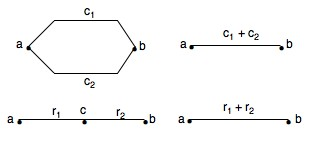
\includegraphics[width=2.5in]{addr.jpg} 
   \caption{Conductances add in parallel, resistances add in series.}
   \label{addr}
\end{figure}


In Figure~\ref{addr} voltages $ v(a), v(b) $ are prescribed, as are conductances $ c_1, c_2 $ and resistances $ r_1, r_2 $.
 In the top two diagrams  
the current flowing from $ a $ to $ b $ is clearly
\[ (v(a)-v(b))(c_1 + c_2). \]
 In the bottom  left diagram  direct calculation shows the induced voltage at $ c $ is 
\[ 
\frac{ \frac{1}{r_1} v(a) + \frac{1}{r_2} v(b) } { \frac{1}{r_1} + \frac{1}{r_2} }.
\]
Easy calculation then shows the current flowing out of $ a $, and the current flowing into $ b $, is 
\[
\frac{v(a) - v(b)}{r_1 + r_2} 
\]
in both of the bottom diagrams. 

It follows that in any circuit the two left side diagrams can be replaced by the corresponding right side diagrams when computing induced voltages, current flow or effective resistance



See [DS, p 44] for an example calculation.



%%%%%%%%%%%%%%%%%%%%%%%%%%%%%%%%
%%%%%%%%%%%%%%%%%%%%%%%%%%%%%%%%
%%%%%%%%%%%%%%%%%%%%%%%%%%%%%%%%
\section{\textbf{Random Walk Interpretation of a Graph}}\label{rwi}

\subsection{Definition of the RW on G}  This is characterised by defining the probability of moving from $ x $ to $ y $ to be
\begin{equation} \label{}
p_{xy} = \frac{c_{xy}}{c_x}.
\end{equation}
Thus \emph{rows} of the \emph{transition matrix} $ P:= (p_{xy})_{x\in V, y\in V}  $ are probability vectors, with row $ x $ containing the probabilities of leaving node $ x $.

The RW always begins at time $ 0 $, and its position at time $ n \geq 0 $ is denoted by~$ X_n $.

 \subsection{Markov Chain}  The random walk is a markov chain with state space $ V   $  and transition probabilities $ p_{xy} $.
\begin{itemize}
\item The markov chain is \emph{irreducible} since $ G $ is connected, and so any state can be reached from any other state.  

\item Hence by standard markov chain theory there is a \emph{unique steady state distribution} $ (w_x)_{x\in V } $.

\item As for any markov chain, if $ (u_x)_{x\in V} $ is the probability distribution at one time then $ (v_x)_{x\in V} $, where $ v_x = \sum_y   u_y p_{yx} $, gives the probability distribution at the next time.

\item It follows by direct calculation
 that the \emph{steady state distribution $ w_x $ is proportional to $ c_ x $},%
\footnote{Since if $ w_x:= c_x/C$ then
\[
 \sum_y w_y p_{yx}  = \sum_y \frac{c_y}{C} \frac{c_{yx}}{c_y} = \sum_y\frac{c_{yx}}{C} = 
      \sum_y\frac{c_{xy}}{C} = \frac{c_x}{C} = w_x. 
\]
Hence  $ w_x $ is the steady state distribution by uniqueness.}
 and  so   
\begin{equation} \label{}
 w_x = \frac{c_x}{C}. 
\end{equation} 
      
  \item The markov chain is \emph{reversible}, i.e.
  \[ w_x p_{xy} = w_y p_{yx} \quad  \forall x,y\in V .\]
  
  \item \emph{Interpretation of reversibility}: One cannot tell the direction of time by watching the RW evolve from the steady state distribution $ w $.  More precisely
 \begin{align*}
  P(xy)  := &\  P(X_0=x) \, P(X_1=y | X_0=x)  
  = w_x p_{xy} 
  \\  = &\ w_y p_{yx}   
   =  P(X_0=y) \, P(X_1=x | X_0=y )   =: P(yx).
  \end{align*} 
  
  Similarly 
\begin{align*} 
   P(x_0x_1\dots x_n) &= w_{x_0} p_{x_0 x_1} p_{x_1 x_2} \cdots p_{x_{n-1} x_n}\\
  & = w_{x_n} p_{x_n x_{n-1}} \cdots p_{x_2 x_1} p_{x_1 x_0}
  = P(x_n  \dots x_1x_0 ) .
\end{align*} 
  
  The following equivalent version does not explicitly refer to the steady state distribution.  For any path $ x_0 x_1 \dots x_n $
  and beginning at each end respectively, 
  \[  c_{x_0} P^{x_0}( x_0 x_1 \dots x_n ) =  c_{x_n} P^{x_n}( x_n  \dots x_1x_0 ). \]
  
  \item Conversely, any reversible markov chain is the RW given by a graph, provided we allow $ c_{xx}> 0 $.%
  \footnote{Suppose the markov chain is $ p $ and the steady state distribution is $ w $. Then $ w_x p_{xy} = w_y p_{yx} \ \forall x,y $.  Define $ c_{xy} = w_x p_{xy} $ and note $ c_{xy} = c_{yx} $. Moreover,
  \[ \frac{c_{xy}}{c_x} = \frac{c_{xy}}{\sum_z c_{xz}} = \frac{w_x p_{xy}}{\sum_z w_x p_{xz}} = p_{xy}, \]
  and so this gives the original markov chain.
  }
  
  \item The natural measure on $ V $  is $ (c_x)_{x\in V} $.  The corresponding \emph{transition density}  is defined  for $ x \sim y $ by  
  \[  p(x,y) := \frac{P^x(X_1=y) }{c_y}   = \frac{c_{xy}}{c_x c_y} = \frac{P^y(X_1=x) }{c_x}  = p(y,x).\]
  Reversibility thus is equivalent to symmetry of the transition density $ p(x,y) $ (but \emph{not} of~$ p_{xy} $). 
\end{itemize} 
 
%%%%%%%%%%%%%%%%%%%%%%%%%%%%%%%%%%%
\subsection{Three quantities associated with the RW}
These are  important and continually arise.

Suppose $ \emptyset \neq \partial V \subset V $.  Think of $ \partial V $ as a ``boundary set'' of nodes.

\begin{itemize} 

\item Suppose $ f : \partial V \to \mathbb{R} $ is given. Suppose $ x \in V $.  Then
\begin{equation} \label{}
\mathbb{E}^x f(X_{T_{\partial V}})
\end{equation} 
is the ``expected pay-off'', where $ {T_{\partial V}} $ is the time of first arrival at $ \partial V $.

If $ x \in \partial V $ then $ T_{\partial V}=0 $ and so $    f(X_{T_{\partial V}}) =f(x) $.

In this section $ \partial V = \{a,b\} $, $ f(a) = a $ and $ f(b) = 0 $, and so $ \mathbb{E}^x f(X_{T_{\partial V}})
= P^x(T_a < T_b ) $.
 In Section~\ref{secfc}, both $ \partial V =B $ and $ f $ are arbitrary.

\item Suppose $ a  \notin \partial V $.  Then
\begin{equation} \label{} 
   \mathbb{E}^a (V_{x\to \partial V})
\end{equation}
is the expected number of times, starting at $ a $,  that the walk hits $ x $ \emph{before} reaching $ \partial V $. 

 If $ x = a $ then \emph{the initial visit at time $ 0 $ is included} as a visit.

If $ x \in \partial V $ then $ V_{x\to \partial V} = 0 $.
 
 In this section $ \partial V = \{ b \} $. In Section~\ref{secfc}, $ \partial V =B $ is arbitrary.
 
 \item Suppose $ a  \notin \partial V $.  Then
 \begin{equation} \label{} 
 P^a (T_{\partial V}  < T^+_a )
\end{equation}  
is the probability the walk reaches $\partial V$ without returning to $  a $.

The notation $ T^+_a $ denotes the first \emph{return} time to $ a $, i.e.\ the first visit \emph{after} time $ 0$.
It is also called the \emph{escape probability} from $ a $ to $ \partial V $.
\end{itemize} 

\begin{proposition} For $ a \notin \partial V $,
\begin{equation} \label{epr}  
\boxed{
\mathbb{E}^a  V_{a\to \partial V }  = 1/P^a (T_{\partial V} < T^+_a).
}
\end{equation} 
\end{proposition} 

\begin{proof}  Let
\begin{align*}
p &= P^a (T_{\partial V} < T^+_a)  \quad \text{(i.e.\ ``success'')},\\
1-p &= P^a (T^+_a< T_{\partial V})  \quad \text{(i.e.\ ``failure'')}.
\end{align*}
The  number of ``failures'' before a success is  a geometric distribution with parameter $ p $.  That is,  the probability of exactly $ n $ returns to $ a $ before reaching ${\partial V} $, or equivalently exactly $ n+1 $ visits,  is $ (1-p)^n p $.  Hence the expected number of visits to $  a $ before reaching $  \partial V $ is  $1$ $  + $ the mean of the geometric distribution, and  so by a standard result%
\footnote{To see this directly let $ Z $ denote the number of visits to $ a $ before first reaching $  \partial V  $. Then 
\begin{align*}
\mathbb{E} (Z) &= \sum_{n\geq 0} (n+1) (1-p)^n p 
 =-p\sum_{n\geq 0} \frac{d}{dp}(1-p)^{n+1}  \\
& = -p \frac{d}{dp}\sum_{n\geq 0}(1-p)^{n+1}   
 = -p\frac{d}{dp}\left(\frac{1-p}{p} \right)  =\frac{1}{p}.
\end{align*}
}
  is $ 1+ (1-p)/p = 1/p$.
  \end{proof} 

\emph{Remark}:  The preceding also follows from the electric network interpretation; see \eqref{ec1} and \eqref{ec2} for the case~$ \partial V = \{ b\}$.


%%%%%%%%%%%%%%%%%%%%%%%%%%%%%%%%%%%
\subsection{Harmonic Extensions} \label{har}

Consider the RW previously described. Fix $ a\neq b \in V $.  For $ x 
\in V $ define
 \begin{gather}
 \boxed{h(x)  = P^x(T_a < T_b),}\label{dfh}\\
\boxed{g(x)  
=  \frac{1}{c_x}\, \mathbb{E}^a (V_{x\to b}).} \label{dfg}
\end{gather}
 


Clearly
\begin{equation} \label{bchg} 
\begin{gathered}
h(a) = 1, \ h(b) = 0;\\
g(a) = \frac{1}{c_a} \mathbb{E}^a V_{a\to b},
\  g(b) = 0.
\end{gathered} 
\end{equation} 
Moreover,  see ~\eqref{dlap} for the definition of $ \lap $,
\begin{equation} \label{}
\boxed{
\lap h = 0, \quad \lap g = 0 , \quad x \neq a,b .
}
\end{equation} 

\begin{proof} Because every visit to $ x $ is \emph{followed} by a visit to some  $y \sim  x $,
\begin{equation} \label{} 
h(x)   = \sum_y p_{xy} P^y (T_a < T_b) 
   = \sum_y \frac{c_{xy}}{c_x} \, h(y) ;
\end{equation} 
and because every visit to $ x $ is \emph{preceded} by a visit to some $ y \sim x $,%
\footnote{More precisely, fix $ x \neq a,b $. Then
\begin{align*}
g(x) &= \frac{1}{c_x} \mathbb{E}^a  (V_{x\to b}) 
      =  \frac{1}{c_x} \sum_{n \geq 1} P^a(X_n = x)\quad \text{(as  $x \neq a $) } \\
     &=  \frac{1}{c_x} \sum_{n \geq 1} \sum_{y\sim x} P^a(X_{n-1} = y) p_{yx} 
     =  \frac{1}{c_x}  \sum_{y\sim x} \frac{c_{yx}}{c_y}\, \mathbb{E}^a  (V_{y\to b}) 
     =   \sum_{y\sim x}  \frac{c_{xy}}{c_x}  g(y).
 \end{align*}
    }
\begin{equation} \label{hhg}
 \begin{aligned} 
 g(x) &:= \frac{1}{c_x}   \mathbb{E}^a V_{x\to b} = 
  \frac{1}{c_x} \sum_y p_{yx}\,  \mathbb{E}^a V_{y\to b}\\
 & = \sum_y\frac{1}{c_x}\, \frac{c_{yx}}{c_y} \, c_y\, g(y) =  \sum_y \frac{c_{xy}}{c_y}  g(y).  
\end{aligned} 
\end{equation}   \qedhere
\end{proof}   

\mbox{}


Note that \emph{reversibility is needed for $ g $ to be harmonic}, but not so for $ h $.

\medskip For later purposes (this is generalised and becomes the definition of the Green's function at $ a $ in~\eqref{dfgf}) note also that 
\begin{equation} \label{lhg}
\boxed{
-\lap g(a) = \frac{1}{c_a} .
} 
\end{equation} 
\begin{proof}
By the same calculation as in~\eqref{hhg} after noting
\[
g(a)   := \frac{1}{c_a}   \mathbb{E}^a V_{a\to b} = 
  \frac{1}{c_a} +  \frac{1}{c_a}\sum_y p_{ya}\,  \mathbb{E}^a V_{y\to b},
  \]
where the second equality is because every visit to $ a $ except for the first is preceded by a visit to some~$ y \sim a $.
\end{proof} 

 

%%%%%%%%%%%%%%%%%%%%%%%%%%%%%%%%%%%%%%%%%
%%%%%%%%%%%%%%%%%%%%%%%%%%%%%%%%%%%%%%%%%
%%%%%%%%%%%%%%%%%%%%%%%%%%%%%%%%%%%%%%%%%
%%%%%%%%%%%%%%%%%%%%%%%%%%%%%%%%%%%%%%%%%
\section{\textbf{Connection between EN and RW}} \label{secER}


\subsection{Interpretation of  $ h $} \label{bvh}
By definition,
\[ h(x) = P^x(T_a < T_b) .\]
Hence $ h $ is the unique voltage   (i.e.\ harmonic function) $ h $ with $ h(a)= 1 $ and $ h(b) = 0 $.

Moreover, the flux $ i_a $ through the network and hence the \emph{effective conductance} $ \mathbb{C}_{ab} $ is%
\begin{equation} \label{ec1}
\boxed{\mathbb{C}_{ab}  (:= i_a/h(a)) = i_a := -c_a \lap h(a) = c_a   P^a(T_b < T^+_a) = c_a/\mathbb{E}^aV_{a\to b} .}
\end{equation} 

\begin{proof}
\begin{align*}
i_a &:=  c_a \lap h(a) = \sum_x\big(h(a) -h(x) \big) c_{ax}  \\
& =\sum_x \big(1-P^x(T_a < T_b)\big)c_{ax} \\
&=c_a\sum_x  p_{ax} P^x(T_b < T_a)  
  = c_aP^a(T_b < T^+_a).
\end{align*}
For the last equality use \eqref{epr}. 
\end{proof} 
 

%%%%%%%%%%%%%%%%%
\subsection{Interpretation of  $ g $}  By definition
\[
g(a) = \frac{1}{c_a} \mathbb{E}^a  V_{a\to b},
\quad g(b) = 0 .
\]
So $ g $ is the unique harmonic function (voltage) with these boundary values.

More interestingly, the \emph{current along each edge} $ xy $ is
\begin{equation} \label{nt}
\boxed{i_{xy} = \mathbb{E}^a(\text{net no of traverses from   $x $ to $ y $ before $ b $}).}
\end{equation} 

\begin{proof}
\begin{align*}
i_{xy} &= (g(x)-g(y) )c_{xy}  \\
  & = \frac{c_{xy}}{c_x} \mathbb{E}^a(V_{x\to b}) 
     -  \frac{c_{xy}}{c_y} \mathbb{E}^a(V_{y\to b}) 
  =p_{xy}\mathbb{E}^a(V_{x\to b}) 
     -  p_{yx}\mathbb{E}^a(V_{y\to b}) \\
     &=  \mathbb{E}^a(\text{no.\ of traverses from  $ x $ to $ y $})  - 
     \mathbb{E}^a(\text{no.\ of traverses from  $ y $ to $ x $}) \\
     &=  \mathbb{E}^a(\text{\emph{net} no.\ of traverses from  $ x $ to $ y $ before $ b $}). 
     \end{align*} 
\end{proof}

It then follows that the flux (current) through the network  is
\begin{equation} \label{ucn} 
\boxed{ i_a = \sum_x i_{ax} =  \mathbb{E}^a(\text{\emph{net} no.\ of traverses out of $ a $}) = 1. }
\end{equation} 
 It now follows that the \emph{effective conductance} of $ G $ is
\begin{equation} \label{ec2}
\boxed{ \mathbb{C}_{ab}\ (:= i_a/v(a)) = c_a / \mathbb{E}^a V_{a\to b} = c_a P^a (T_b < T^+_a),}
\end{equation} 
with the last equality from~\eqref{epr}. 

\subsection{Relation between $ h $ and $ g $}Since $ h(x)/g(x) = h(a)/g(a) $, from \eqref{dfh}, \eqref{dfg} and \eqref{ec2},
\begin{equation} \label{} 
\boxed{h(x) = \mathbb{C}_{ab} g(x) 
, \quad \text{i.e.} \ 
 P^x (T_a < T_b) = 
\frac{\mathbb{C}_{ab}}{c_x}\,  \mathbb{E}^aV_{x\to b}.}
\end{equation} 

\emph{Note}: The proofs of~\eqref{ec1} and \eqref{ec2} give a non probabilistic proof of~\eqref{epr}. 


%%%%%%%%%%%%%%%%%%%%%%%%%
%%%%%%%%%%%%%%%%%%%%%%%%%
%%%%%%%%%%%%%%%%%%%%%%%%%

\section{\textbf{Crossing Time, Einstein Relation}}
%%%%%%%%%%%%%%%%%%%%%%%%%
\subsection{Crossing Time Theorem} [Chandra et al, 1989]
\begin{equation} \label{ctt} 
\boxed{\mathbb{E}^a T_b + \mathbb{E}^b T_a = \mathbb{R}_{ab}\, C(G).}
\end{equation} 

\begin{proof}%
\footnote{I havn't seen quite this proof before, but it is natural with the current development.}
 Starting from any point $ a $,
\[    T_b = \sum_x V_{x\to b}.\]
It follows from the harmonicity of $ g $ in Section~\ref{har} that 
\begin{align*}
\mathbb{E}^a T_b  &= \sum_x \mathbb{E}^a (V_{x\to b}) = \sum c_x    \frac{ \mathbb{E}^a (V_{x\to b})   }{c_x} \\
    &= \sum_x c_x \big(\text{harmonic ext $ v(x) $ to $ V $ of $ v(a) = \frac{\mathbb{E}^a (V_{a\to b})}{c_a}$},  v(b) = 0 \big) \\
    &= \frac{\mathbb{E}^a (V_{a\to b})}{c_a} \sum_x c_x \big(\text{harmonic ext $ v(x) $ to $ V $ of } v(a) = 1 ,  v(b) = 0  \big) \\
    &= \mathbb{R}_{ab}  \sum_x c_x \big(\text{harmonic ext $ v(x) $ to $ V $ of } v(a) = 1, v(b) = 0 \big) .
\end{align*} 
Similarly, using the previously proved $ \mathbb{R}_{ab} = \mathbb{R}_{ba}$,
\[
\mathbb{E}^b T_a  =  \mathbb{R}_{ab}  \sum_x c_x \big(\text{harmonic ext $ v(x) $ to $ V $ of $ v(a) = 0 ,\  v(b) = 1$} \big) .
\]
Adding, and using the uniqueness of harmonic extension,
\begin{align*}
\mathbb{E}^a T_b + \mathbb{E}^b T_a &=  \mathbb{R}_{ab} \sum_x c_x \big(\text{harmonic ext $ v(x) $ to $ V $ of $ v(a) = 1 ,\  v(b) = 1$} \big) \\
&=  \mathbb{R}_{ab} \sum_x c_x  
 = \mathbb{R}_{ab}\, C(G). \qedhere
\end{align*} 
 \end{proof}

%%%%%%%%%%%%%%%%%%%%%%%%%%
\subsection{Einstein Relation}
The left side of  \eqref{ctt} is the expected \emph{commute time} from $ a $ to $ b $ and back, $ \mathbb{R}_{ab}$ is the distance between $ a $ and $ b $ in the resistance metric, and $ C = C(G)$ is the total mass of $G $ (see page~\pageref{tm}).  
This  gives the multiplicative version of the \emph{Einstein relation}:  
\begin{equation} \label{er1}
\boxed{\text{Time} = \text{Distance} \times \text{Mass}.}
\end{equation} 

We often have a ``scale'' or parameter $ x $, such as Euclidean distance, where for appropriate exponents
\begin{equation} \label{dexp} 
 \text{Time} \sim x^{d_w},  
\text{ Distance} \sim x^{d_r}, \text{ Mass} \sim x^{d_f }. 
\end{equation} 
More precisely:  ``Time'' is the commute time between points which are separated by Euclidean distance $\approx  x $,
``Distance'' is the  resistance metric distance  between points which are separated by Euclidean distance $\approx  x $,  and ``Mass'' is the mass of a ball whose Euclidean diameter is $\approx  x $.

The exponents are called the \emph{walk dimension} $ d_w $, the \emph{resistance dimension}  $ d_r $,
and the \emph{fractal dimension}  $ d_f $.  

From \eqref{er1} and \eqref{dexp} one gets the usual form of the \emph{Einstein relation}:
\begin{equation} \label{}
\boxed{d_w = d_r + d_f.}
\end{equation} 


%%%%%%%%%%%%%%%%%%%%%%%%%%%%%%%%%%%%%%%
\subsection{Triangle Inequality} Here is a random  walk proof of the triangle inequality for the resistance metric.  This also gives the error term, see Footnote~\ref{rwet}.

\begin{proof}  \label{rwp} Clearly%
\footnote{\label{rwet}Using an obvious notation, $ T^a_c = T^a_b + T^b_c $  if $T^a_b \leq  T^a_c $ and $ T^a_c = T^a_b - T^c_b < T^a_b + T^b_c$ if $ T^a_c < T^a_b $.  So $ T^a_c \leq T^a_b + T^b_c $ in both cases.

More precisely,
\begin{align*}
\mathbb{E}^a T_c &= P^a(T_b \leq T_c)\, \mathbb{E}^a(T_c \mid T_b \leq T_c )
     + P^a(T_c < T_b)\,  \mathbb{E}^a(T_c \mid T_c < T_b )  \\     
     & = P^a(T_b \leq T_c)\,  (\mathbb{E}^aT_b + \mathbb{E}^bT_c )   + 
          P^a(T_c < T_b)\, \big(\mathbb{E}^aT_b + \mathbb{E}^bT_c - 
                                               (\mathbb{E}^bT_c  + \mathbb{E}^cT_b  )\big)\\
     &=  (\mathbb{E}^aT_b + \mathbb{E}^bT_c ) - P^a(T_c < T_b) \mathbb{E}^b_c ,
\end{align*} 
where $  C^b_c =   C^c_b :=  T^b_c  +  T^c_b $ is the   \emph{commute time} from $  $ to $ c  $ and back to $ b $, and $ \mathbb{E}^b_c := \mathbb{E} C^b_c $.
} 
\[ \mathbb{E}^aT_c    \leq  \mathbb{E}^aT_b + \mathbb{E}^bT_c.
\]
Switching $ a $ and $ c $ and adding,
\[
\mathbb{E}^aT_c  +  \mathbb{E}^cT_a  \leq  \mathbb{E}^aT_b + \mathbb{E}^bT_a + \mathbb{E}^bT_c  + \mathbb{E}^cT_b.
\]
Dividing both sides by $ C(G) $ and using the crossing time inequality~\eqref{ctt} gives 
\[    
\mathbb{R}_{ac} \leq \mathbb{R}_{ab}  + \mathbb{R}_{bc} . \qedhere
\] 
\end{proof} 









%%%%%%%%%%%%%%%%%%%%%%%%%%%%%%%%
%%%%%%%%%%%%%%%%%%%%%%%%%%%%%%%%
%%%%%%%%%%%%%%%%%%%%%%%%%%%%%%%%
%%%%%%%%%%%%%%%%%%%%%%%%%%%%%%%%
%%%%%%%%%%%%%%%%%%%%%%%%%%%%%%%%
%%%%%%%%%%%%%%%%%%%%%%%%%%%%%%%%

\section{\textbf{Further Connections between EN and RW}}  \label{secfc} Consider a non empty set of ``boundary'' nodes $   B = \partial V \subset V $.  This generalises the situation in Sections~\ref{secEN}, \ref{rwi} and~\ref{secER}, where $ \partial V = \{a,b\} $ or $ \partial V = \{ a \} $. 

\subsection{Dirichlet Problem}

(This is analogous to the classical P.D.E.\ problem.%
\footnote{\label{char}Let $ \Omega \subset \mathbb{R}^n $ be  non empty bounded and open with a ``nice'' boundary 
$ \partial \Omega $, e.g.\ $ C^1 $.  
Suppose $h : \partial V \to \mathbb{R}   $ is prescribed and also ``nice'', e.g.\ $ C^1 $.  Then there is a unique harmonic extension of $ h $ to $ \Omega $.   
})
Suppose $  h : \partial V \to \mathbb{R}   $ is prescribed.  Then there exists a unique extension of $ h $ to $ V^\circ $ satisfying
\begin{equation} \label{}
\lap h(x) = 0  \quad x \in V^\circ .
\end{equation}
Uniqueness, and hence existence, follow as in Section~\ref{mf}.

\medskip
\emph{RW Interpretation}:  (This is analogous to the case of Brownian Motion in the P.D.E.\ setting.%
\footnote{If $ X $ is Brownian motion on $ \Omega $ and $ T_{\partial \Omega} $ is the time of first reaching the boundary, then 
\[
\phi(x) = \mathbb{E}^x \phi(X_{T_{\partial \Omega}}).
\]
})
The solution 
 $ h $   is the expected ``payoff'':
\begin{equation} \label{harw}
 \boxed{h(x) =  \mathbb{E}^xh(X_{T_{\partial V}}) ,}
\end{equation} 
 where $ {T_{\partial V}} $ is the time of first arrival at $ \partial V $.
 The fact that $ h $ agrees with the given boundary values, and is harmonic   on $ V^\circ $, is given by the same argument as in Section~\ref{har}.
 
\medskip \emph{EN Interpretation}:
 It also follows as in Sections~\ref{pm} and \ref{mf} that we can regard $ h $ as giving the voltage  at each node in  $ V $ for  the prescribed voltages on $ \partial V $.

%%%%%%%%%%%%%%%%%%%%%%%%%%%%%%%%%
\subsection{Green's Function} Fix $ a \in V^\circ $.  Motivated by the classical situation%
\footnote{Suppose $ a \in \Omega $.  Then the Green  function $ \mathcal{G}_a(x) = \mathcal{G} (x,a)$ is characterised  for $x \in  \overline{\Omega} $ by
\begin{align*}
-\lap \mathcal{G}_a(x) &=    \delta_a(x) \quad  \text{if } x \in  \Omega, \quad \text{(Dirac delta measure, equality in distributional sense)}\\ 
 \mathcal{G}_a(x)& = 0 \quad \text{if } x \in \partial \Omega.
 \end{align*} 
 
 In particular, 
 \[
 \mathcal{G}_a(x) = \begin{cases} -\frac{\ln |x-a| }{2\pi} + \psi(x) & n=2, \\
                                                              \frac{c_n}{|x-a|^{n-2}}  + \psi(x) & n \geq 3, \ (c_3 = \frac{1}{4\pi})
                                                              \end{cases}
                                                              \]
 where $ \psi(x) $ is the unique harmonic function on $ \Omega $ such that $  \mathcal{G}_a(x)  = 0$ if $ x \in \partial \Omega$.
 
The solution of 
\begin{align*}
-\lap u & = f \quad \text{in } \Omega \\
 u &= 0 \quad \text{on } \partial \Omega
 \end{align*} 
 is then given by the following ``weighted sum'' of Green functions:
 \[
 u(x) = \int_{\Omega} \mathcal{G}_y(x) f(y)\,  dy.
 \]
 
 \emph{Symmetry} of Green's function is shown  for $ a\neq b \in \Omega $ as follows:
 \[
 \mathcal{G}_a(b) - \mathcal{G}_b(a) =
 \int_\Omega \mathcal{G}_b \lap \mathcal{G}_a    - \mathcal{G}_a  \lap \mathcal{G}_b 
 = \int_{\partial \Omega}  \mathcal{G}_b   \frac{\partial \mathcal{G}_a }{\partial \nu}
        -       \mathcal{G}_a   \frac{\partial \mathcal{G}_b }{\partial \nu} = 0
        \]
The first and third equalities are  from the definition of $ \mathcal{G}_a $ and $ \mathcal{G}_b $. The second is  by Green's formula.       Strictly, one should integrate over $ \Omega \setminus (B_\epsilon (a) \cup B_\epsilon (a)) $ and let $ \epsilon \to 0 $.
  }
\emph{Green's function centred at $ a $} is the unique function $ \mathcal{G}_a:V\to \mathbb{R}  $ given by
\begin{equation} \label{dfgf}
\begin{gathered}
           \boxed{ -\lap \mathcal{G}_a(x) = \dfrac{1}{c_a} \mathcal{X}_a(x),} \quad x \in V^\circ,\\
            \mathcal{G}_a(x)  = 0 \quad x \in \partial V,
   \end{gathered}
\end{equation} 
where $ \mathcal{X}_a $ is the characteristic function equal to $ 1 $ at $ a $ and $ 0$  elsewhere.
Uniqueness, and hence existence, follow as in Section~\ref{mf}.

Note that $ \dfrac{1}{c_a} \mathcal{X}_a $ is the natural choice as the ``Dirac measure'' centred at $ a $ since it integrates to $ 1  $ w.r.t.\ the natural measure $ (c_x)_{x\in V }$.


%-\lap \mathcal{G}_a(x) &= \begin{cases} \dfrac{1}{c_a} & x=a \\
%                                                                        0    & x\neq a,\  x \in V^\circ
%                                             \end{cases} \\
%                                  \mathcal{G}_a(x) &= 0 \qquad x \in \partial V,



\medskip \emph{Symmetry} of Green's function 
\begin{equation} \label{} 
\boxed{\mathcal{G}_b(a) =  \mathcal{G}_a(b),} \quad a,b\in V^\circ,
\end{equation}
 follows immediately from Green's identity~\eqref{gi}, which is just an algebraic calculation.  In fact 
\[  (\lap \mathcal{G}_a, \mathcal{G}_b) = (\mathcal{G}_a, \lap \mathcal{G}_b) ,\]
where each side is the natural inner product with the weighting $ c_x $ at $ x $.  The left side is $ c_a \mathcal{G}_b(a) \dfrac{1}{c_a}  = \mathcal{G}_b(a) $ and the right side is similarly $ \mathcal{G}_a(b) $.


\medskip
\emph{RW Interpretation}:  We claim 
\begin{equation} \label{wig}
\boxed{\mathcal{G}_a(x) = \frac{1}{c_x} \mathbb{E}^a V_{x\to \partial V } .}  
\end{equation}  
To see this,  one verifies that if $ \mathcal{G}_a $ is defined in this way then the conditions in~\eqref{dfgf} are all satisfied.   The argument is the same as for~\eqref{lhg}, \eqref{hhg} and \eqref{bchg}, respectively.  The main point is that every visit to $ x $, except for the first if $ x=a $,  is preceded by a visit to a neighbour of $ x $.
 
\medskip \emph{EN Interpretation}: 

\begin{center} \fbox{For an  applied voltage $ \mathcal{G}_a   $, $ i_a = 1 $.}\end{center}

That is, if the voltage $ \mathcal{G}_a   $ is applied at $ \{a\} \cup \partial V $ then a unit current flows out of $ a $ into the network, and hence out of the network via $ \partial V $. 
This follows as in~\eqref{ucn}, using~\eqref{nt}; the main point is that using~\eqref{ilap},  $ i_a =  -c_a \mathcal{G}_a(a) = 1 $.
 
\medskip
\emph{Poisson's equation}: The solution of 
\begin{equation} \label{}
\begin{aligned}
- \lap u (x) &= f (x) \quad x \in V^\circ, \\
u(x) &= 0 \quad x \in \partial V,
\end{aligned}
\end{equation}
is given by 
\begin{equation} \label{}
\boxed{u(x) = \sum_{y\in V^\circ} \mathcal{G}_y(x)  f(y)\, c_y.}
\end{equation}
\begin{proof} If $ x \in \partial V $ then
\[
       \sum_{y\in V^\circ} \mathcal{G}_y(x)  f(y)\, c_y = 0 ,
       \]
 and if $ x \in V^\circ $ then
\[-\lap_x \left(  \sum_{y\in V^\circ} \mathcal{G}_y(x)  f(y)\, c_y \right) =
       \sum_{y\in V^\circ} \frac{\mathcal{X}_y(x)}{c_y} f(y) c_y = f(x).
       \]
\end{proof}        
%%%%%%%%%%%%%%%%%%%%%%%%%%%%%%%%%%%%%
%%%%%%%%%%%%%%%%%%%%%%%%%%%%%%%%%%
\subsection{Effective Resistance} \label{secer}Let $ B = \partial V  $. Motivated by the previous RW and EN interpretations and by Ohm's law (resistance = voltage/current), the \emph{effective resistance} $ \mathbb{R}_{aB} $ is defined in any of the equivalent ways
\begin{enumerate}

\item \emph{Analytic version}: \fbox{$ \mathbb{R}_{aB} =  \mathcal{G}_a(a) $} where $  \mathcal{G}_a(x) $ is the solution of~\eqref{dfgf}.

\item \emph{RW version}: \fbox{$  \mathbb{R}_{aB}= \dfrac{1}{c_a} \mathbb{E}^a V_{a\to \partial V} 
   = \Big(c_aP^a(T_{\partial V} < T_a^+) \Big)^{-1} $,}
    where the last equality is from~\eqref{epr}. 

\item  \emph{EN version}:   
    \fbox{\parbox{7cm}{$   \mathbb{R}_{aB} $ is the voltage at $ a $ such that  zero voltage   at $ B $ then induces a unit   flow  from $ a $ to $ B $.}}
 
\end{enumerate} 


%%%%%%%%%%%%%%%%%%%%%%%%%%%%%%%
%\subsection{Alternate RW version of Effective Resistance and Green's Function}
%  Let $ h_a $ be the harmonic extension to $ V \setminus (B\cup \{a\} ) $ of the function given by 
%$ h_a(a)=1 $ and $ h_a(b) = 0 $ for $ b \in B $.

%Then $  \mathcal{G}$ is a multiple of $ h_a $ and so
%\[
%\frac{\mathcal{G}_a(x)}{h_a(x)} = \begin{cases}
%                \dfrac{ \mathcal{G}_a(a)}{h_a(a)}  = \mathcal{G}_a(a) = \mathbb{R}_{aB} \\
%                \dfrac{-\lap\mathcal{G}_a(a)}{-\lap h_a(a)}  = \dfrac{1/c_a}{-\lap h_a(a)}
%                \end{cases}
%\]
%The bottom line comes from the fact that for any $ f $, $ \lap f(a) $ is a linear combination of $ f(x) $ for $ x \sim a $.

%Note that
%\begin{equation} \label{}
%- \lap h_a(a) =   P^a(T_B < T^+_a ) 
%\end{equation}
%by the argument in the proof of \eqref{ec1}. 

%\medskip It follows:
%\begin{equation} \label{} 
%\begin{aligned} 
% \mathbb{R}_{aB}^{-1} &=  \mathbb{C}_{aB} = c_a P^a(T_B < T^+_a),  \\
%\mathcal{G}_a(x) &= \mathbb{R}_{aB} h_a(x) = \mathbb{R}_{aB} P^x(T_a < T_B ) .
%\end{aligned} 
%\end{equation} 


%%%%%%%%%%%%%%%%%%%%%%%%%%%%%%%%
%%%%%%%%%%%%%%%%%%%%%%%%%%%%%%%%
%%%%%%%%%%%%%%%%%%%%%%%%%%%%%%%%
\section{\textbf{Matrices}}
In a later section we give a slightly different, more general  and more ``modern'' approach via matrices.  This section is an extension of material in [DS].

\subsection{Goals}
Fix the boundary set $ \partial V \subset V $. 
Using matrices we want to compute 
\begin{enumerate}
\item the harmonic extension of a given boundary  function $ h: \partial V \to \mathbb{R} $;
\item   the Green function $ \mathcal{G}_a(x) $ for $ a \in V^\circ $ and $ x \in V $;  
\item the effective resistance $ \mathbb{R}_{ab} $ between any two vertices $ a,b \in V $;


\item  the expected number of hits on $ x $ by the RW starting at $ a $ and before it reaches $ \partial V$   (i.e.\  just~$ c_x \mathcal{G}_a(x) $);
\item the expected crossing time from $ a $ to $ \partial V $;
\item  the probability that the RW from $ a $ first hits $ \partial V $ at   $ b \in \partial V $.
\end{enumerate} 



\subsection{Important Matrices}�  
Consider  the markov chain with $ m $ absorbing states  $ \partial V $, $ n $ other states $ V^\circ $, and transition probabilities given by the RW.

Let  $ \widetilde{P} $ be the \emph{transition matrix} for the RW \emph{with absorbing states $ \partial V $}:
\begin{equation} \label{tma} 
 \widetilde{P} =   \begin{bmatrix}  
      I & O \\
      R & Q  
 \end{bmatrix},
\end{equation}    
where
\begin{itemize}
  \item 
 \[
 \widetilde{P}_{xy} =  \begin{cases}
  c_{xy}/c_x  & \text{ if } x\in V^\circ,\ y\in V,\\
  \delta_{xy} & \text{ if } x \in \partial V, \ y\in V. 
 \end{cases}
 \]

\item $  I = I_m$ is the $ m \times m $ identity matrix corresponding to the $ m $ boundary nodes; 
\item $ R  $ is $ n \times m $, $ Q $ is $ n \times n$, and they correspond to the probabilities of passing from  the $ n $ interior nodes  
 to boundary nodes and interior nodes respectively.
 \end{itemize}
 
\medskip
The \emph{limit behaviour} of the markov chain is
\begin{equation} \label{}
\lim_{k\to \infty} \widetilde{P}^k = \begin{bmatrix} I_m & O  \\ B & O \end{bmatrix},
\end{equation} 
either by direct calculation%
\footnote{Note $ P^k = \begin{bmatrix} I_m & O \\
                                        (I_n + Q +\dots +Q^{k-1}) R & \  Q^k 
                                        \end{bmatrix} $.
 } 
 or from \eqref{hb}.


 
\medskip The \emph{fundamental matrix} is 
\begin{equation} \label{fma}
\boxed{N  := (I_n -Q)^{-1} }= I_n + Q+ Q^2 + Q^3 + \cdots.
\end{equation} 
It follows that
 \begin{equation} \label{fm}
\boxed{N_{xy} = \mathbb{E}^xV_{y\to \partial V},} \quad x,y \in V^\circ.
\end{equation}
since
\begin{equation} \label{} 
(Q^k)_{xy}  = P^x(\text{being at $ y $ on the $ k$th step}).
\end{equation} 

\medskip The \emph{crossing time vector} is
\begin{equation} \label{} 
\boxed{ t_x := \mathbb{E}^xT_{\partial V}} 
= \sum_y N_{xy}, \quad x \in V^\circ.
\end{equation} 
Thus 
\begin{equation} \label{}
\boxed{t = N1_n}
\end{equation}
where $ 1_n $ is the vector of $ n $ units.



\medskip  The \emph{boundary hitting probability  matrix} is
\begin{equation} \label{hb}
\boxed{B_{xb} := P^x(\text{hitting boundary at $ b $}),} \quad x\in V^\circ,\ b \in \partial V.
\end{equation}
Hence from \eqref{fm},
\begin{equation} \label{}
\boxed{B = NR  = (I_n-Q)^{-1}R .}
\end{equation} 

\medskip This computes Goals (4), (5) and (6).

\subsection{Harmonic Extension, Green's Function, Effective Resistance}\mbox{}

\subsubsection{Harmonic Extension}  Since from~\eqref{harw} the harmonic extension of $ h : \partial V \to \mathbb{R} $ is given by
$ h(x) = \mathbb{E}^x h(X_{T_{\partial V}}) $, it follows from~\eqref{hb} that 
\begin{equation} \label{}
\boxed{h_{V^\circ} = B h_{\partial V} = (I_n - Q)^{-1}R\, h_{\partial V}.}
\end{equation}

An alternative proof is to note that $ h $ is characterised by  
\[
 \begin{bmatrix} h_{\partial V  } \\ h_{V^\circ} \end{bmatrix}
 =   \begin{bmatrix} I & O \\ R & Q   \end{bmatrix}
       \begin{bmatrix} h_{\partial V  } \\h_{V^\circ} \end{bmatrix},
\] 
and so 
\[
h_{V^\circ}= (I_n - Q)^{-1}R\, h_{\partial V}  = B h_{\partial V} .
\]


\subsubsection{Green's Function}   Since
$ \mathcal{G}_a(x) = \frac{1}{c_x} \mathbb{E}^aV_{x\to \partial V } $ 
from \eqref{wig}, it follows from~\eqref{fm} that
\begin{equation} \label{}
\begin{gathered}
\boxed{\mathcal{G}_a(x)  =  N_{ax}/c_x,}\  x\in V^\circ, \\
\mathcal{G}_a(x)  =   0,\  x\in \partial V,
\end{gathered}
\end{equation} 

\subsubsection{Resistance Metric}   Since $ \mathbb{R}_{aB} = \frac{1}{c_a} \mathbb{E}^aV_{a\to B} $ from Section~\ref{secer}, it follows from~\eqref{fm}  that if we take $ \partial V = B $  then 
\begin{equation} \label{}
\boxed{\mathbb{R}_{aB} = \frac{N_{aa}}{c_a}. }
\end{equation}
Of particular interest  is $ B = \{ b \} $.

\bigskip
 This computes Goals (1), (2) and (3).


%%%%%%%%%%%%%%%%%%%%%%%%%%%%%%%%
%%%%%%%%%%%%%%%%%%%%%%%%%%%%%%%%
%%%%%%%%%%%%%%%%%%%%%%%%%%%%%%%%
\section{\fbox{\textbf{Partial Summary So Far}}}

\subsection{Laplacian} 

Suppose $ f : V \to \mathbb{R} $. 
\begin{enumerate}

\item \emph{Analytic version}: $ \lap f(x)  := \sum_y \dfrac{c_{xy}}{c_x} (f(y) - f(x)) $.
\item \emph{RW version}:  $ \lap f(x) = \mathbb{E}^x f(X_1) - f(x) $.
\item \emph{EN version}: $ \lap f(x) = -\dfrac{i_x}{c_x} $ where $ i_x := \sum_y c_{xy} (f(y) - f(x) ) $ is the current flowing out of $ x $ if the voltage at each $ x\in V $ is $ f(x) $.
\item \emph{LA version}:%
\footnote{``LA'' for ``Linear Algebra''.}
$ \lap f = (P-I) f $ where $ (P_{xy})  =  (c_{xy}/c_x) $ is the transition matrix.
\end{enumerate}  


%%%%%%%%%%%%%%%%%%%%%%%%%%%%%%%%%%
\subsection{Harmonic Extension}
Suppose $ h :\partial V \to \mathbb{R} $ is prescribed.
\begin{enumerate}

\item \emph{Analytic version}:  $ \exists $ a unique extension to $ h : V \to \mathbb{R} $ such that $ \lap h = 0 $ on $ V^\circ $.
\item \emph{RW version}: $ h(x) = \mathbb{E}^x h(X_{T_{\partial V}}) $ for $ x \in V $.
\item  \emph{EN version}:  $ h $ is the voltage induced on $ V= V^\circ \cup \partial V  $ when a voltage $ h(v) $ is applied to each $ v \in \partial V $.
(Mathematically, the induced voltage is characterised by prescribing Ohm's law on each edge and Kirchoff's law on each interior node.)
\item \emph{LA version}:  With transition matrix $ 
 \widetilde{P} =   \begin{bmatrix}  
      I_m & O \\
      R & Q  
 \end{bmatrix} $ as in~\eqref{tma},  $ h_{V^\circ} = (I_n-Q)^{-1}R\, h_{\partial V} $.
 \end{enumerate} 
  
%%%%%%%%%%%%%%%%%%%%%%%%%%%%%%%%%%
\subsection{Green's Function}  \label{secgf} Suppose $ \emptyset \neq \partial V \subset V $ and  $ b \in V^\circ $.  Then the Green function \mbox{$ \mathcal{G}_a : V \to \mathbb{R} $} is characterised as follows:
\begin{enumerate}
\item \emph{Analytic version}: $ \exists $ a unique function $ \mathcal{G}_a  $ such that 
\begin{align*}
-\lap \mathcal{G}_a(x) &= \begin{cases} 1/ c_a  & x=a \\
                                                                        0    & x\neq a,\  x \in V^\circ
                                             \end{cases} \\
                                  \mathcal{G}_a(x) &= 0 \qquad x \in \partial V .
   \end{align*}
   
\item \emph{RW versions}:  $ \mathcal{G}_a(x) = \dfrac{1}{c_x} \mathbb{E}^a V_{x\to \partial V} 
 = \mathbb{R}_{aB}  P^x(T_a < T_{\partial V} )$ for $ x \in V $.

\item  \emph{EN version}:  $ \mathcal{G}_a(a)$ is the voltage to apply at  $ a $ such that if zero voltage is applied at each $ b \in \partial V $ then unit current flows out of $ a $, through the network  and out of $ \partial V $.  $ \mathcal{G}_a(x)$ is the induced voltage at each $ x \in V ^\circ $.

\item \emph{LA version}: $ \mathcal{G}_a $ is obtained from row $ a $ of the fundamental matrix $ N : = (I_n - Q)^{-1} $ via 
\[ 
\mathcal{G}_a(x)  
= \begin{cases}   N_{ax}/c_x & x\in V^\circ, \\
                               0   & x\in \partial V.
                             \end{cases}
\]
\end{enumerate} 

%%%%%%%%%%%%%%%%%%%%%%%%%%%%%%%%%%
\subsection{Effective Resistance} \label{secer2}Let $ B = \partial V  $. Motivated by (3) in Section~\ref{secgf} and Ohm's law (resistance = voltage/current), the effective resistance $ \mathbb{R}_{aB} $ is defined as in 93) below and so characterised as follows:
\begin{enumerate}

\item \emph{Analytic version}: $ \mathbb{R}_{aB} =  \mathcal{G}_a(a) $ where $  \mathcal{G}_a(x) $ is the solution of (1) in Section~\ref{secgf}.

\item \emph{RW versions}: $  \mathbb{R}_{aB}= \dfrac{1}{c_a} \mathbb{E}^a V_{a\to \partial V} 
=  \big(c_a P^a(T_B < T^+_a)\big)^{-1}$.

\item  \emph{EN version}:  $   \mathbb{R}_{aB} $ is the voltage required at $ a $, if   voltage zero is applied at $B $, in order that a unit current flow  from $ a $ to $ B $.

\item \emph{LA version}: $   \mathbb{R}_{aB} =  \dfrac{1}{c_a}  N_{aa}$.

\end{enumerate} 


%%%%%%%%%%%%%%%%%%%%%%%%%%%%%%%%
%%%%%%%%%%%%%%%%%%%%%%%%%%%%%%%%
%%%%%%%%%%%%%%%%%%%%%%%%%%%%%%%%
\section{\textbf{Matrix Examples}}

All computations done in Maple.  See accompanying worksheet.

\subsection{One dimensional RW} Consider the simple RW of Figure~\ref{RWex}. Here $ V = \{0,1,2,3,4\} $.  Let $ \partial V = \{0,4\}   $   or $\partial V = \{ 4\}$. 

\begin{figure}[htbp] %  figure placement: here, top, bottom, or page
   \centering
   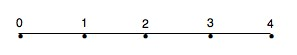
\includegraphics[width=3in]{RWex.jpg} 
   \caption{A simple random walk}
   \label{RWex}
\end{figure}

Then one computes respectively:
\begin{gather*}
\widetilde{P} =\  \begin{matrix}
      {} & \begin{matrix} 0&4&1&2&3 \end{matrix}  \\ 
    \begin{matrix} 0\\4\\1\\2\\3 \end{matrix}
   &
    \begin{bmatrix} 1 & 0 & 0 & 0 & 0 \\
                                    0 & 1 & 0 & 0 & 0 \\
                      \frac{1}{2} & 0 & 0 & \frac{1}{2} & 0 \\
                      0 & 0 & \frac{1}{2} & 0  & \frac{1}{2}  \\
                      0 & \frac{1}{2} & 0  & \frac{1}{2} & 0 
        \end{bmatrix}
   \end{matrix},\
N =   \  \begin{matrix}
          {} & \begin{matrix}  1&2&3 \end{matrix}  \\ 
     \begin{matrix}  1\\2\\3 \end{matrix}
    &      
    \begin{bmatrix} \frac{3}{2}   & 1 & \frac{1}{2}  \\
                                                              1 & 2  &1 \\
                      \frac{1}{2} & 1 & \frac{3}{2} 
        \end{bmatrix}
  \end{matrix}
,\
 t =\  \begin{matrix}
  \begin{matrix} 1  \\ 2 \\ 3   \end{matrix}
&
  \begin{bmatrix} 3  \\ 4 \\ 3   \end{bmatrix}
\end{matrix}
,\
   B = \  \begin{matrix}
   {} & \begin{matrix} 0&4  \end{matrix}  \\ 
  \begin{matrix} 1  \\ 2 \\ 3   \end{matrix}
&   
     \begin{bmatrix} \frac{3}{4}   &  \frac{1}{4}  \\
                                         \frac{1}{2}  &  \frac{1}{2}  \\
                      \frac{1}{4} &  \frac{3}{4} 
        \end{bmatrix}
\end{matrix} ;       
\\   \\ %%%%%%%%%%%%%%%%%%%%%%%%%%%%
\widetilde{P} =\  \begin{matrix}
      {} & \begin{matrix} 4&0&1&2&3 \end{matrix}  \\ 
    \begin{matrix} 4\\0\\1\\2\\3 \end{matrix}
   &
    \begin{bmatrix} 1 & 0 & 0 & 0 & 0 \\
                                    0 & 0 & 1 & 0 & 0 \\
                     0 & \frac{1}{2}  & 0 & \frac{1}{2} & 0 \\
                      0 & 0 & \frac{1}{2} & 0  & \frac{1}{2}  \\
                      \frac{1}{2} & 0 & 0  & \frac{1}{2} & 0 
        \end{bmatrix}
   \end{matrix},\
N =   \  \begin{matrix}
          {} & \begin{matrix}  0 &1&2&3 \end{matrix}  \\ 
     \begin{matrix}  0 \\1\\2\\3 \end{matrix}
    &      
    \begin{bmatrix} 4  & 6 & 4 &2  \\
                                3 & 6  &4 & 2\\
                      2 & 4 & 4  & 2 \\
                       1 & 2 & 2 & 2 
        \end{bmatrix}
  \end{matrix},\
 t =\  \begin{matrix}
  \begin{matrix} 0  \\ 1  \\ 2 \\ 3   \end{matrix}
&
  \begin{bmatrix} 16  \\ 15 \\ 12 \\ 7     \end{bmatrix}
\end{matrix},\
   B = \  \begin{matrix}
   {} & 4 \\ 
  \begin{matrix} 0 \\ 1  \\ 2 \\ 3   \end{matrix}
&   
     \begin{bmatrix} 1 \\ 1  \\ 1 \\ 1   \end{bmatrix}
\end{matrix}.        
\end{gather*}
 

\bigskip From this one reads off, for $ x,y\in V^\circ $ and $ b \in \partial V $,
\begin{align*}
\mathbb{E}^x V_{y\to \partial V} &= N_{xy} \\
\mathbb{E}^x T_{\partial V} &= t_x \\
P^x (X_{T_{\partial V}}  = b ) &= B_{xb}\\
\text{harmonic extension of $ h_{\partial V}$: } h_{V^\circ} &= B h_{\partial V} \\
\mathcal{G}_x(y) &= N_{xy}/c_y \\
\mathbb{R}_{xB}    &= N_{xx}/c_x\\
P^y(T_x< T_{\partial V}) &= \frac{\mathbb{C}_{xB}}{c_y} N_{xy}.
\end{align*} 

In particular, 
\begin{align*}
\mathbb{E}^0T_4 &=  \text{(by symmetry) } \mathbb{E}^4T_0 = 16 \\
\mathbb{R}_{0,4} &= 4/1 = 4\\
C(G) &= 1 + 2 + 2 + 2 + 1 = 8.
\end{align*} 
Note that this satisfies the crossing time theorem $ \mathbb{E}^0T_4 +  \mathbb{E}^4T_0 = \mathbb{R}_{0,4}\, C(G) $.




%%%%%%%%%%%%%%%%%%%%%%%%%%%
\subsection{Simple Triangle   T  }

Consider the triangle network with unit resistances in Figure~\ref{triex}.   First with $ \partial V = \{0\}   $   and then with $\partial V = \{0,1\}$.  
\begin{figure}[htbp] %  figure placement: here, top, bottom, or page
   \centering
   \includegraphics[width=1.5in]{TrI.jpg} 
   \caption{A simple triangle}
   \label{triex}
\end{figure}

One computes respectively:

\begin{gather*}
\widetilde{P} =  
   \begin{bmatrix} % or pmatrix or bmatrix or Bmatrix or ...
      1 & 0 & 0 \\
      \frac{1}{2}  & 0 & \frac{1}{2}    \\
      \frac{1}{2} & \frac{1}{2} & 0
   \end{bmatrix} , \
N =    \begin{bmatrix} % or pmatrix or bmatrix or Bmatrix or ...
      \frac{4}{3} & \frac{2}{3} \\
      \frac{2}{3} & \frac{4}{3}  \\
   \end{bmatrix},\
   t =    \begin{bmatrix} % or pmatrix or bmatrix or Bmatrix or ...
         2 \\
         2 
      \end{bmatrix}, \
      B =  \begin{bmatrix} % or pmatrix or bmatrix or Bmatrix or ...
         1 \\
         1 
      \end{bmatrix};
\\ \\%%%%%%%%%%%%%%%%%%%%%%%%%
\widetilde{P} =  
   \begin{bmatrix} % or pmatrix or bmatrix or Bmatrix or ...
      1 & 0 & 0 \\
      0 & 1 & 0    \\
      \frac{1}{2} & \frac{1}{2} & 0
   \end{bmatrix} , \
N =   1,\
   t = 1, \
      B =  \begin{bmatrix} % or pmatrix or bmatrix or Bmatrix or ...
         \frac{1}{2}  & \frac{1}{2} 
      \end{bmatrix}.
\end{gather*}

In particular \label{Tq}
\begin{align*}
\mathbb{E}^2T_0 &= t_2 = 2 \text{ (top row)}\\
\mathbb{E}^2 T_{ \{0,1\}} &= t_2 = 1  \text{ (bottom row)}\\
\mathbb{R}_{0,2}  = \mathbb{R}_{2,0}    &=\frac{4/3}{2}  =  \frac{2}{3}\\
\mathbb{R}_{2,\{0,1\}}    &=\frac{1}{2}\\
C(G) &=   2 + 2 + 2   = 6.
\end{align*} 
The crossing time theorem  $ \mathbb{E}^0T_2 +  \mathbb{E}^2T_0 = \mathbb{R}_{0,2}\, C(G) $ is satisfied.


%%%%%%%%%%%%%%%%%%%%%%%%%%%
\subsection{SG(2) prefractal} \label{secsg2}  The network is shown in Figure~\ref{SG(2)}.  Each of the 6 edges is given unit resistance.

\begin{figure}[htbp] %  figure placement: here, top, bottom, or page
   \centering
   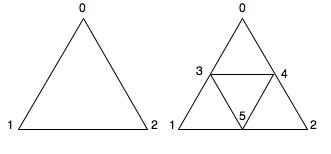
\includegraphics[width=3in]{SG(2).jpg} 
   \caption{The $ SG(2)$  prefractal}
   \label{SG(2)}
\end{figure}

We consider the three cases $ \partial V = \{0\}, \{0,1\}, \{0,1,2\} $. Then one computes respectively:
{\allowdisplaybreaks
\begin{gather*}
 \widetilde{P} =   \begin{bmatrix}  
      1 & 0 & 0 & 0 & 0 & 0  \\
      0 & 0 & 0 & \frac{1}{2}  & 0 &  \frac{1}{2}  \\
      0 & 0 & 0 & 0 & \frac{1}{2} &  \frac{1}{2}  \\
      \frac{1}{4}  &  \frac{1}{4} & 0 & 0 &  \frac{1}{4} &  \frac{1}{4}  \\
       \frac{1}{4} & 0 &  \frac{1}{4} &  \frac{1}{4} & 0 & \frac{1}{4}  \\
      0 &  \frac{1}{4} &  \frac{1}{4} &  \frac{1}{4} &  \frac{1}{4} & 0  \\
        \end{bmatrix},\
 N=  \begin{bmatrix}  
      \frac{20}{9}  & \frac{10}{9}  &\frac{20}{9}   &\frac{16}{9}  & \frac{8}{3}    \\
      \frac{10}{9}  & \frac{20}{9}  &\frac{16}{9}   &\frac{20}{9}  & \frac{8}{3}    \\
      \frac{10}{9}  & \frac{8}{9}  &\frac{22}{9}   &\frac{14}{9}  &2    \\
      \frac{8}{9}  & \frac{10}{9}  &\frac{14}{9}   &\frac{22}{9}  & 2  \\
       \frac{4}{3} &  \frac{4}{3} &  2  &  2 &  \frac{10}{3}   \\
        \end{bmatrix},\   
    t=       \begin{bmatrix} 10\\10\\8\\8\\10\\ \end{bmatrix},\ 
    B=    \begin{bmatrix} 1 \\1  \\ 1\\1\\1\\ \end{bmatrix} ;
\\ \\
 \widetilde{P} =   \begin{bmatrix}  
      1 & 0 & 0 & 0 & 0 & 0  \\
      0 & 1 & 0 & 0 & 0 & 0  \\
      0 & 0 & 0 & 0 & \frac{1}{2} &  \frac{1}{2}  \\
      \frac{1}{4}  &  \frac{1}{4} & 0 & 0 &  \frac{1}{4} &  \frac{1}{4}  \\
       \frac{1}{4} & 0 &  \frac{1}{4} &  \frac{1}{4} & 0 & \frac{1}{4}  \\
      0 &  \frac{1}{4} &  \frac{1}{4} &  \frac{1}{4} &  \frac{1}{4} & 0  \\
        \end{bmatrix},\
 N=  \begin{bmatrix}  
      \frac{5}{3}  & \frac{2}{3}  &\frac{4}{3}   &\frac{4}{3}        \\
      \frac{1}{3}  & \frac{4}{3}  &\frac{2}{3}   &\frac{2}{3}        \\
      \frac{2}{3}  & \frac{2}{3}  &\frac{26}{15}   &\frac{14}{15}        \\
      \frac{2}{3}  & \frac{2}{3}  &\frac{14}{15}   &\frac{26}{15}       \\
        \end{bmatrix},\   
   t =          \begin{bmatrix} 5 \\3  \\ 4\\4\\
         \end{bmatrix},\ 
    B=       \begin{bmatrix} \frac{1}{2} & \frac{1}{2} \\
                                          \frac{1}{2} & \frac{1}{2} \\
                                          \frac{3}{5} & \frac{2}{5} \\
                                          \frac{2}{5} & \frac{3}{5} \\
                                           \end{bmatrix}  ;
 \\ \\
 \widetilde{P} =   \begin{bmatrix}  
      1 & 0 & 0 & 0 & 0 & 0  \\
      0 & 1 & 0 & 0 & 0 & 0  \\
      0 & 0 & 1 & 0 & 0 & 0  \\
      \frac{1}{4}  &  \frac{1}{4} & 0 & 0 &  \frac{1}{4} &  \frac{1}{4}  \\
       \frac{1}{4} & 0 &  \frac{1}{4} &  \frac{1}{4} & 0 & \frac{1}{4}  \\
      0 &  \frac{1}{4} &  \frac{1}{4} &  \frac{1}{4} &  \frac{1}{4} & 0  \\
        \end{bmatrix},\
 N=  \begin{bmatrix}  
      \frac{6}{5}  & \frac{2}{5}  &\frac{2}{5}         \\
      \frac{2}{5}  & \frac{6}{5}  &\frac{2}{5}         \\
      \frac{2}{5 }  & \frac{2}{5}  &\frac{ 6}{ 5}          \\
        \end{bmatrix},\   
   t =          \begin{bmatrix} 2 \\2  \\ 2\\
         \end{bmatrix},\ 
    B=       \begin{bmatrix}     
     \frac{2}{5}  & \frac{2}{5}  &\frac{1}{5}         \\
      \frac{2}{5}  & \frac{1}{5}  &\frac{2}{5}         \\
      \frac{1}{5 }  & \frac{2}{5}  &\frac{ 2}{ 5}          \\
                                           \end{bmatrix}  .
\end{gather*}
}

In particular
\begin{align*}
\mathbb{E}^1T_0 &= t_1 = 10 \text{ (top row)}\\
\mathbb{E}^2 T_{ \{0,1\}} &= t_2 = 5  \text{ (middle row)}\\
\mathbb{R}_{0,1}  = \mathbb{R}_{1,0}    &= N_{11}/ c_1 = 
                                      \frac{20/9}{2}  =  \frac{10}{9}  \text{ (top row)}\\
\mathbb{R}_{2,\{0,1\}}    &= N_{22}/ c_2 = 
                                      \frac{5/3}{2}  =  \frac{5}{6}  \text{ (middle row)}\\
C(G) &=   3 \times 2 + 3\times 4  = 18.
\end{align*} 
The crossing time theorem  $ \mathbb{E}^0T_1 +  \mathbb{E}^1T_0 = \mathbb{R}_{0,1}\, C(G) $ is again satisfied.

\medskip
\emph{Mass, Time and Resistance Scaling}:  \label{sc2} Since edges all have unit resistance, i.e.\  the network is simple, the mass is $ \sum_x \text{degree}(x) $, or equivalently twice the number of edges, or equivalently 6 times the number of triangles, i.e.\ 18. But the mass of $ T $ is 6.  So the mass scaling $ m $ is \mbox{$ 18/3 = 6$}.

Next compare the crossing  times and effective resistances above with those for $ T $ on page~\pageref{Tq}. 
Let  $ \tau $ and $ \rho $, respectively, denote the factors by which 
 the  walk times and resistance between comparable nodes scale up in passing from $ T $ to $ SG(2) $.
 
 Then 
$  m = 18/6=3$, $ \tau = 10/2 \text{ or }    5/1 = 5$,
and $  \rho =   \frac{10}{9}\Big/\frac{2}{3} \text{ or } 
                                     \frac{5}{6}\Big/\frac{1}{2}      =\frac{5}{3}$.
That is:
\begin{equation} \label{} 
\boxed{m = 3,\  \tau = 5,\  \rho = 5/3.}
\end{equation} 
 
 Note the Einstein relation
$  \tau = m \times \rho $ 
holds.                                     


%%%%%%%%%%%%%%%%%%%%%%%%%%%
\subsection{SG(3) prefractal}  \label{secsg3} The network is shown in Figure~\ref{SG(3)}.  Each of the 18 edges is given unit resistance.


\begin{figure}[htbp] %  figure placement: here, top, bottom, or page
   \centering
   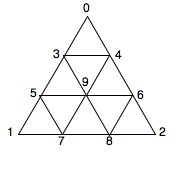
\includegraphics[width=2in]{SG(3).jpg} 
   \caption{The $ SG(3)$  prefractal}
   \label{SG(3)}
\end{figure}

We consider the two cases $ \partial V = \{0\}, \{0,1\} $. Then one computes respectively:
{
\allowdisplaybreaks
\begin{gather*}
 \widetilde{P} =   \begin{bmatrix} 
 1 & 0 & 0  & 0 & 0  & 0 & 0  & 0 & 0 & 0 \\
 0 & 0 & 0  & 0 & 0 & \frac{1}{2}   &0 & \frac{1}{2}  & 0  & 0\\
 0 & 0 & 0  & 0 & 0  & 0 & \frac{1}{2}   & 0 & \frac{1}{2}  & 0 \\
 \frac{1}{4}  & 0 & 0  & 0 &  \frac{1}{4}   &  \frac{1}{4}  & 0  & 0 & 0 &  \frac{1}{4}  \\
 \frac{1}{4}  & 0 & 0  &  \frac{1}{4}  & 0  & 0 & \frac{1}{4}   & 0 & 0 &  \frac{1}{4}  \\
 0 &  \frac{1}{4}  & 0  &  \frac{1}{4}  & 0  & 0 & 0  &  \frac{1}{4}  & 0 &  \frac{1}{4}  \\
 0 & 0 &  \frac{1}{4}   & 0 &  \frac{1}{4}   & 0 & 0  & 0 &  \frac{1}{4}  &  \frac{1}{4}  \\
 0 &  \frac{1}{4}  & 0  & 0 & 0  &  \frac{1}{4}  & 0  & 0 &  \frac{1}{4}  &  \frac{1}{4}  \\
 0 & 0 &  \frac{1}{4}   & 0 & 0  & 0 & \frac{1}{4}   &  \frac{1}{4}  & 0 &  \frac{1}{4}  \\
 0 & 0 & 0  &  \frac{1}{6}  & \frac{1}{6}  & \frac{1}{6} & \frac{1}{6}  & \frac{1}{6} & \frac{1}{6} & 0 \\
 \end{bmatrix},\
N =  \left[ \begin {array}{ccccccccc} {\frac {20}{7}}&{\frac {10}{7}}&{
\frac {44}{21}}&{\frac {40}{21}}&{\frac {76}{21}}&\frac{8}{3}&{\frac {80}{21}}
&{\frac {64}{21}}&{\frac {30}{7}}\\\noalign{\medskip}{\frac {10}{7}}&{
\frac {20}{7}}&{\frac {40}{21}}&{\frac {44}{21}}&\frac{8}{3}&{\frac {76}{21}}&
{\frac {64}{21}}&{\frac {80}{21}}&{\frac {30}{7}}\\\noalign{\medskip}{
\frac {22}{21}}&{\frac {20}{21}}&{\frac {17}{7}}&{\frac {11}{7}}&{
\frac {15}{7}}&{\frac {13}{7}}&{\frac {43}{21}}&{\frac {41}{21}}&3
\\\noalign{\medskip}{\frac {20}{21}}&{\frac {22}{21}}&{\frac {11}{7}}&
{\frac {17}{7}}&{\frac {13}{7}}&{\frac {15}{7}}&{\frac {41}{21}}&{
\frac {43}{21}}&3\\\noalign{\medskip}{\frac {38}{21}}&\frac{4}{3}&{\frac {15}{
7}}&{\frac {13}{7}}&{\frac {83}{21}}&{\frac {53}{21}}&{\frac {23}{7}}&
{\frac {59}{21}}&{\frac {29}{7}}\\\noalign{\medskip}\frac{4}{3}&{\frac {38}{21
}}&{\frac {13}{7}}&{\frac {15}{7}}&{\frac {53}{21}}&{\frac {83}{21}}&{
\frac {59}{21}}&{\frac {23}{7}}&{\frac {29}{7}}\\\noalign{\medskip}{
\frac {40}{21}}&{\frac {32}{21}}&{\frac {43}{21}}&{\frac {41}{21}}&{
\frac {23}{7}}&{\frac {59}{21}}&\frac{13}{3}&{\frac {23}{7}}&{\frac {31}{7}}
\\\noalign{\medskip}{\frac {32}{21}}&{\frac {40}{21}}&{\frac {41}{21}}
&{\frac {43}{21}}&{\frac {59}{21}}&{\frac {23}{7}}&{\frac {23}{7}}&\frac{13}{3}
&{\frac {31}{7}}\\\noalign{\medskip}{\frac {10}{7}}&{\frac {10}{7}}&2
&2&{\frac {58}{21}}&{\frac {58}{21}}&{\frac {62}{21}}&{\frac {62}{21}}
&{\frac {34}{7}}\end {array} \right], 
\\
t =  \left[ \begin {array}{c} {\frac {180}{7}}\\\noalign{\medskip}{\frac {
180}{7}}\\\noalign{\medskip}17\\\noalign{\medskip}17
\\\noalign{\medskip}{\frac {167}{7}}\\\noalign{\medskip}{\frac {167}{7
}}\\\noalign{\medskip}{\frac {179}{7}}\\\noalign{\medskip}{\frac {179}
{7}}\\\noalign{\medskip}{\frac {162}{7}}\end {array} \right] ,\
B =  \left[ \begin {array}{c} 1\\\noalign{\medskip}1\\\noalign{\medskip}1
\\\noalign{\medskip}1\\\noalign{\medskip}1\\\noalign{\medskip}1
\\\noalign{\medskip}1\\\noalign{\medskip}1\\\noalign{\medskip}1
\end {array} \right] ;
 \end{gather*}
 }
and
 {\allowdisplaybreaks
\begin{gather*}
 \widetilde{P} =   \begin{bmatrix} 
1 & 0 & 0  & 0 & 0  & 0 & 0  & 0 & 0 & 0 \\
 0 & 1 & 0  & 0 & 0 & 0  &0 &0 & 0  & 0\\
 0 & 0 & 0  & 0 & 0  & 0 & \frac{1}{2}   & 0 & \frac{1}{2}  & 0 \\
 \frac{1}{4}  & 0 & 0  & 0 &  \frac{1}{4}   &  \frac{1}{4}  & 0  & 0 & 0 &  \frac{1}{4}  \\
 \frac{1}{4}  & 0 & 0  &  \frac{1}{4}  & 0  & 0 & \frac{1}{4}   & 0 & 0 &  \frac{1}{4}  \\
 0 &  \frac{1}{4}  & 0  &  \frac{1}{4}  & 0  & 0 & 0  &  \frac{1}{4}  & 0 &  \frac{1}{4}  \\
 0 & 0 &  \frac{1}{4}   & 0 &  \frac{1}{4}   & 0 & 0  & 0 &  \frac{1}{4}  &  \frac{1}{4}  \\
 0 &  \frac{1}{4}  & 0  & 0 & 0  &  \frac{1}{4}  & 0  & 0 &  \frac{1}{4}  &  \frac{1}{4}  \\
 0 & 0 &  \frac{1}{4}   & 0 & 0  & 0 & \frac{1}{4}   &  \frac{1}{4}  & 0 &  \frac{1}{4}  \\
 0 & 0 & 0  &  \frac{1}{6}  & \frac{1}{6}  & \frac{1}{6} & \frac{1}{6}  & \frac{1}{6} & \frac{1}{6} & 0 \\
 \end{bmatrix},\
N =  \left[ \begin {array}{cccccccc} {\frac {15}{7}}&\frac{6}{7}&{\frac {8}{7}}&\frac{6}{7}
&{\frac {16}{7}}&{\frac {8}{7}}&{\frac {16}{7}}&{\frac {15}{7}}
\\\noalign{\medskip}\frac{3}{7}&{\frac {523}{315}}&{\frac {55}{63}}&{\frac {
257}{315}}&{\frac {277}{315}}&{\frac {41}{63}}&{\frac {263}{315}}&{
\frac {10}{7}}\\\noalign{\medskip}\frac{4}{7}&{\frac {55}{63}}&{\frac {113}{63
}}&{\frac {41}{63}}&{\frac {79}{63}}&{\frac {43}{63}}&{\frac {65}{63}}
&{\frac {11}{7}}\\\noalign{\medskip}\frac{3}{7}&{\frac {257}{315}}&{\frac {41}
{63}}&{\frac {523}{315}}&{\frac {263}{315}}&{\frac {55}{63}}&{\frac {
277}{315}}&{\frac {10}{7}}\\\noalign{\medskip}{\frac {8}{7}}&{\frac {
277}{315}}&{\frac {79}{63}}&{\frac {263}{315}}&{\frac {853}{315}}&{
\frac {65}{63}}&{\frac {587}{315}}&{\frac {15}{7}}\\\noalign{\medskip}
\frac{4}{7}&{\frac {41}{63}}&{\frac {43}{63}}&{\frac {55}{63}}&{\frac {65}{63}
}&{\frac {113}{63}}&{\frac {79}{63}}&{\frac {11}{7}}
\\\noalign{\medskip}{\frac {8}{7}}&{\frac {263}{315}}&{\frac {65}{63}}
&{\frac {277}{315}}&{\frac {587}{315}}&{\frac {79}{63}}&{\frac {853}{
315}}&{\frac {15}{7}}\\\noalign{\medskip}\frac{5}{7}&{\frac {20}{21}}&{\frac {
22}{21}}&{\frac {20}{21}}&{\frac {10}{7}}&{\frac {22}{21}}&{\frac {10}
{7}}&{\frac {19}{7}}\end {array} \right] , \\
t =  \left[ \begin {array}{c} {\frac {90}{7}}\\\noalign{\medskip}{\frac {
53}{7}}\\\noalign{\medskip}{\frac {59}{7}}\\\noalign{\medskip}{\frac {
53}{7}}\\\noalign{\medskip}{\frac {83}{7}}\\\noalign{\medskip}{\frac {
59}{7}}\\\noalign{\medskip}{\frac {83}{7}}\\\noalign{\medskip}{\frac {
72}{7}}\end {array} \right] ,\
B =  \left[ \begin {array}{cc} \frac{1}{2} &\frac{1}{2} \\\noalign{\medskip}{\frac {19}{30}}
&{\frac {11}{30}}\\\noalign{\medskip}\frac{2}{3} &\frac{1}{3} \\\noalign{\medskip}{
\frac {11}{30}}&{\frac {19}{30}}\\\noalign{\medskip}{\frac {8}{15}}&{
\frac {7}{15}}\\\noalign{\medskip}\frac{1}{3} &\frac{2}{3} \\\noalign{\medskip}{\frac {7
}{15}}&{\frac {8}{15}}\\\noalign{\medskip}\frac{1}{2} &\frac{1}{2} \end {array} \right] .
\end{gather*}
}
 
In particular
\begin{align*}
\mathbb{E}^1T_0 &= t_1 = \frac{180}{7} \text{ (first group)}\\
\mathbb{E}^2 T_{ \{0,1\}} &= t_2 = \frac{90}{7}  \text{ (second group)}\\
\mathbb{R}_{0,1}  = \mathbb{R}_{1,0}    &= N_{11}/ c_1 = 
                                      \frac{20/7}{2}  =  \frac{10}{7}  \text{ (first group)}\\
\mathbb{R}_{2,\{0,1\}}    &= N_{22}/ c_2 = 
                                      \frac{15/7}{2}  =  \frac{15}{14}  \text{ (second group)}\\
C(G) &=   3 \times 2 + 6\times 4  + 6= 36.
\end{align*} 
The crossing time theorem  $ \mathbb{E}^0T_1 +  \mathbb{E}^1T_0 = \mathbb{R}_{0,1}\, C(G) $ is again satisfied! 
 
 \medskip
\emph{Mass, Time and Resistance Scaling}:  \label{sc3}(Compare with $ SG(2) $ for notation.)  For $ SG(3) $ we obtain  the following mass, time and resistance scalings:
$ m =  {36}/{6}=6$,  $   \tau = \frac{180}{7}\Big/2 \text{ or } \frac{90}{7}\Big/ 1 = \frac{90}{7}$  and   
  $ \rho = \frac{10}{7}\Big/\frac{2}{3}  \text{ or } \frac{15}{14}\Big/ \frac{1}{2}  = \frac{15}{7}$.
That is:
\begin{equation} \label{}
\boxed{m = 6,\  \tau = 90/7,\  \rho = 15/7.}
\end{equation} 

 Note the Einstein relation
$  \tau = m \times \rho $ 
holds. 



%%%%%%%%%%%%%%%%%%%%%%%%%%%%%%%%%%%%
%%%%%%%%%%%%%%%%%%%%%%%%%%%%%%%%%%%
%%%%%%%%%%%%%%%%%%%%%%%%%%%%%%%%%%%%%%%
\section{\textbf{Dirichlet Energy}}

\subsection{Definitions}
\begin{itemize}
\item For $ f,g:V\to \mathbb{R} $ define the $\emph{Dirichlet Energy} $ of $ f $, and corresponding bilinear form, by
\begin{equation} \label{def}
\begin{aligned}
\mathcal{E} (f) &= \frac{1}{2} \sum_{x,y} c_{xy}\big(f(x) - f(y)\big)^2,\\
\mathcal{E}(f,g) &= \frac{1}{2}  \sum_{x,y} c_{xy}\big(f(x) - f(y)\big) \big(g(x) - g(y)\big).
\end{aligned}
\end{equation} 
The $ \dfrac{1}{2} $ arises since the energy is ``sitting'' on edges, but each edge appears twice in the sum.

\item \emph{EN Interpretation}: If $ f $ is a voltage then $ i_{xy} = c_{xy} (f(x) - f(y) )$ is the current along the  directed  edge $ xy $ and the first summand in~\eqref{def},
\begin{equation} \label{ened} 
   c_{xy}\big(f(x) - f(y)\big)^2 = i_{xy} \big(f(x) - f(y) \big) = i_{xy}^2 r_{xy},
\end{equation} 
 is the ``energy dissipation'' on the edge $ xy $.  The Dirichlet energy  $ \mathcal{E}(f) $ is the ``energy dissipation'' of the network, or equivalently the energy required to keep the network flowing.
 \end{itemize} 
 
 
 %%%%%%%%%%%%%%%%%%%%%%%%%%%%%%%%%%%
 \subsection{Green's Identity}
(This is analogous to the P.D.E.\  case.) 
\begin{equation} \label{gi}
\mathcal{E}(f,g) = - (\lap f, g) = -( f,\lap g), 
\end{equation}
where $ (h,k) = \sum_x h(x) k(x) c_x $ denotes the $ L^2 $ inner product with the 
 natural measure $ (c_x)_{x\in V} $.
 
 In particular, \emph{$ \lap $ is self-adjoint}.
 
Note that \eqref{gi} expresses the energy $ \mathcal{E}(f)$ as a sum of contributions at \emph{nodes} rather than edges, and the  contribution is $ 0 $ at any node where $ \lap f = 0 $ or $ f=0 $.  
 
\begin{proof}
\begin{align*}
\mathcal{E}(f,g) &= \frac{1}{2} \sum_{x,y} c_{xy} f(x) \big( g(x) - g(y) \big) 
    - \frac{1}{2} \sum_{x,y} c_{xy} f(y) \big( g(x) - g(y) \big) \\
     &= \frac{1}{2} \sum_{x,y} c_{xy} f(x) \big( g(x) - g(y) \big) 
     + \frac{1}{2} \sum_{x,y} c_{yx} f(x) \big( g(x) - g(y) \big) \\
    &= \sum_{x,y} c_{xy} f(x) \big( g(x) - g(y) \big) = -\sum_x f(x)\, \lap g(x)\, c_x.
    \end{align*} 
\end{proof}
 
%%%%%%%%%%%%%%%%%%%%%%%%%%%%%%%%%%% 
\subsection{Thompson's First Principle}  
\begin{proposition}
Suppose $h|_{\partial V} $is  prescribed and $ \lap h = 0 $ on $ V^\circ$.  Then
\[ 
\mathcal{E}(h) = \min \{ \mathcal{E}(f) : f=h \text{ on } \partial V\}.
\]
In the case $ \partial V = \{a,b\} $,   $ \lap h = 0 $ on $ V^\circ $, $ h(a) = 1 $ and $ h(b) = 0 $, then 
\[
\mathcal{E}(h) = \min \{ \mathcal{E}(f) : f(a)=1, f(b)=0\} = \mathbb{C}_{ab}.
\]
\end{proposition} 

The following proof that the Dirichlet minimiser is harmonic  is analogous to the the P.D.E.\ situation.%
 \footnote{(See footnote~\ref{char}.)  The harmonic extension to $\Omega $ of $ h:\partial \Omega \to \mathbb{R} $    is the unique minimiser in $ H^1(\Omega) $ of $ \mathcal{E}(f) := \frac{1}{2} \int_{\Omega} |Df^2 $ with the prescribed boundary conditions.
  Existence comes from taking a minimising sequence and standard P.D.E.\ arguments  to show the sequence converges in the $ H^1 $ sense.   
  
  For here, just note that if $ h $ is harmonic  and $ \phi \in H^1_0(\Omega) $ then 
\begin{align*}
\mathcal{E}(h+\phi) &= \frac{1}{2}\int_{\Omega} |Dh |^2 + 
  \int_{\Omega}  Dh \cdot D\phi  +  \frac{1}{2}\int_{\Omega} |D\phi |^2 \\
&= \mathcal{E}(h)   
  -\int_{\Omega}  \lap h \cdot  \phi  +  \mathcal{E}(\phi) \\
  &= 
  \mathcal{E}(h)    +  \mathcal{E}(\phi)\\
 & \geq  \mathcal{E}(h), \text{ with equality iff $ \phi = 0 $ a.e.}
\end{align*} 
So $ h $ is indeed the unique minimiser.
}
The proof that the Dirichlet energy of the harmonic function is $ \mathbb{C}_{ab} $ follows essentially directly from Green's Identity and the definition of~$ \mathbb{C}_{ab} $.


\begin{proof}  Suppose   $ \phi = 0 $ on $ \partial V $.  Then
\begin{align*}
\mathcal{E}(h+\phi, h+\phi) &= \mathcal{E} (h,h) + 2 \mathcal{E} ( h,\phi) + \mathcal{E}(\phi,\phi)  
                                                  \quad \text{(bilinearity)}\\
&= \mathcal{E}(h,h) - 2 (\lap h,\phi) + \mathcal{E}(\phi,\phi) \quad \text{(Green's identity)}\\
&= \mathcal{E}(h,h)   + \mathcal{E}(\phi,\phi)
\quad \text{(since $ \lap h = 0 $ on $ V^\circ $ and $ \phi = 0 $ on $ \partial V $)}\\
&\geq \mathcal{E}(h,h) 
\end{align*} 
Equality holds in the last line iff $ \phi $ is constant, i.e.\  $ \phi \equiv 0 $. 

This shows that $ h $ is the unique minimiser.


\medskip In the second case, by Green's identity~\eqref{gi},  $ \mathcal{E}(h) =  - c_a \lap h(a) $. 
But  $ - c_a \lap h(a) $ is the current $ i_a $   under the voltage $ h  $, by~\eqref{ilap}.  Since $ h(a) = 1 $ and $ h(b) = 0 $, it follows $ i_a = \mathbb{C}_{ab} $ by the definition of $ C_{ab}$ in~\eqref{effr}. 
\end{proof} 


\subsection{Flows} The following definitions   are motivated by the properties of a current  induced by a voltage applied on $ \partial V $, over a network with possibly unknown conductances.  

\medskip Fix $ \partial V \subset V $.  A \emph{flow} is a function $ j $ on the directed edges of $ G $ such that 
\begin{equation} \label{fld}
\begin{aligned}
j_{xy} & = 0   \text{ for } x \not \sim y \\
j_{xy} &= - j_{yx} \\
\sum_y j_{xy} &= 0 \text{ if }x \in V^\circ .
\end{aligned}
\end{equation}


The \emph{flow out of $ x $} for $ x\in V $ is   
\[  j_x := \sum_y j_{xy} . \]
Hence $ j_x = 0 $ if $ x \in V^\circ $.

The \emph{energy} of $ j $ is 
\begin{equation} \label{}
\mathcal{E}(j) :=  \frac{1}{2} \sum_{x,y} j_{xy}^2 c_{xy}^{-1}. 
\end{equation}

If $ \partial V = \{ a,b\} $ and $ j_a = -j_b = 1 $, then $ j $ is a \emph{unit flow from $ a $ to $ b $}.



%%%%%%%%%%%%%%%%%%%%%%%%%%%%
\subsection{Properties of Flows}  Suppose $ j $ is a flow and $ w:V \to \mathbb{R} $. Then for any function $ w_x $ ,
\begin{equation} \label{prpf} 
\begin{aligned}
\sum_{x\in \partial V} j_x &= 0, \quad    j_a = -j_b \text{ if }  \partial V = \{ a,b\} , \\
\sum_{x,y} (w_x-w_y)j_{xy} &=  2 \sum_{x\in \partial V} w_x j_x .
\end{aligned} 
\end{equation}

\begin{proof} The first line follows from the second with $ w_x \equiv 1 $. 

For the second,
\begin{align*} 
\sum_{x,y} (w_x - w_y) j_{xy} &=   \sum_{x,y} w_x j_{xy} -   \sum_{x,y} w_y j_{xy}  
    =   \sum_{x,y} w_x j_{xy} -   \sum_{x,y} w_x j_{yx}  \\
 &= 2\sum_{x,y} w_x j_{xy}  
   = 2 \sum_x w_x j_x \\ &= 2 \sum_{x\in \partial V} w_x j_x.
  \end{align*}  
\end{proof} 


\subsection{Thompson's Second Principle} 

\begin{proposition} Suppose $ i $ is the unit flow corresponding to a voltage $ v $ applied to $ a $ and $ b $, with $ v(b) = 0 $.  Then 
\[
\mathcal{E}(i) = \min \{ \mathcal{E}(j) :   j \text{ is a unit flow from $ a $ to $ b $}\} = \mathbb{R}_{ab}.
\]
\end{proposition}

The proof of the following is analogous to that for Thompson's first principle. The value of the minimiser follows from that in the first principle by a simple scaling argument.

\begin{proof}
 For feasible $ j $ let $ j_{xy} = i_{xy} + d_{xy}$.  Then $ d_{xy} $ is a flow with $d_a =d_b = 0 $.
Hence
\begin{align*}
\mathcal{E}(j) &= \frac{1}{2} \sum_{x,y} (i_{xy} + d_{xy})^2 r_{xy} \\
   &= \frac{1}{2} \sum_{x,y} i^2_{xy}r_{xy} + \sum_{x,y}i_{xy} d_{xy} r_{xy} + \frac{1}{2} \sum_{x,y}d_{xy}^2r_{xy}.
   \end{align*}
From~\eqref{prpf} the second term on the right equals
\[ 
\sum_{x,y} (v(x)-v(y)) d_{xy} = 2v(a)  d_a + 2v(b) d_b =0.
\]
Hence 
\[
\mathcal{E}(j) \geq \mathcal{E}(i),
\]
with equality iff $ d = 0 $, i.e.\ $ i=j $.

\medskip

If a unit current flows from $ a $ to $ b $ the applied voltage is $  \mathbb{R}_{ab} $, by the definition of $\mathbb{R}_{ab} $. 
But if the applied voltage is $ 1 $ then the Dirichlet energy is $  \mathbb{C}_{ab} $ from Thompson's first principle.  
Hence if the applied  voltage is $ \mathbb{R}_{ab}  $   the Dirichlet energy is multiplied by $  \mathbb{R}_{ab} ^2 $  from the definition~\eqref{def} of Dirichlet energy, since all voltages will then also be scaled up by $ \mathbb{R}_{ab}  $.
That is, 
\[ \mathcal{E}(i) = \mathbb{R}_{ab}^2 \mathbb{C}_{ab} = \mathbb{R}_{ab} .\]
\end{proof} 

%%%%%%%%%%%%%%%%%%%%%%%%%%%%%%%%%%%
\subsection{Cuts and Shorts}
%%%%%%%%%%%%%%%%%%%%%%%%%%%%%%%%
%%%%%%%%%%%%%%%%%%%%%%%%%%%%%%%%
%%%%%%%%%%%%%%%%%%%%%%%%%%%%%%%%
\section{\textbf{Matrices, New Version}}

\subsection{Motivation} 
It is convenient for calculations to write $ \mathcal{E}(f,g) $ as a bilinear form in the standard manner, using a positive semi definite matrix.  This will give a slightly different, but more useful, way of expressing the formula for harmonic extensions and for Green's function.  In particular, we do this in Section~\ref{secTN} concerning trace networks. 

\subsection{Alternative expression for Dirichlet energy}
Note: 
\begin{enumerate}
\item $ \mathcal{E}(f,g)  = \frac{1}{2} \sum_{x,y} c_{xy} (f_x-f_y)(g_x-g_y)$ defines a positive semi definite symmetric bilinear form, and $ \mathcal{E}(f,f) = 0 $ iff $ f $  constant.%
\footnote{Think of the graph of $ \mathcal{E}(f,f) $ as  an  $ n-1 $ dimensional parabola $ \times $ straight line, sitting on $ \mathbb{R}^n$, where $ n $ is the cardinality of $ V $.}

\item  
The terms $ c_{xx}$ are zero.
 Replacing $ c_{xx} $  by any other value will not alter the value of~$ \mathcal{E}(f,g) $.  
 
 \item As for any (positive semi definite) symmetric bilinear form,   $ \mathcal{E}(f,g) =  f^T B g = g^T B f$ for some (positive semi definite) symmetric matrix $ B $.
 
 \item Formula \eqref{de2} expresses the energy as a sum of contributions from   \emph{nodes} rather than edges.

 \end{enumerate} 
 
\medskip  In the following note that $ -A $ is the positive semi definite matrix.
\begin{proposition}
Let $ A = (a_{xy}) $  for $ x,y \in V $, where 
\begin{equation} \label{}
a_{xy} = \begin{cases} c_{xy} & x \neq y \\
                                          -c_x   & x = y 
               \end{cases}.
 \end{equation}
Then 
\begin{equation} \label{de2}
\boxed{\mathcal{E}(f,g) = -\sum_{x,y} a_{xy} f_x g_y}  \ (=  -f^TAg = -g^TAf). 
\end{equation} 
\end{proposition} 

\begin{proof}
 \begin{align*}
\mathcal{E}(f,g) &= \sum_{x,y} c_{xy}f_x g_x - \sum_{x,y} c_{xy} f_x g_y \quad  
                            \text{(since  $ c_{xy}= c_{yx}$)} \\
   &= \sum_{x} c_x f_x g_x - \sum_{\substack{x,y \\ x\neq y}} c_{xy}f_x g_y \quad 
                                         \text{(since  $ c_{x}= \sum_y c_{xy}$ and $ c_{xx} = 0 $)} \\
   &= -\sum_{x} a_{xx} f_x g_x - \sum_{\substack{x,y \\ x\neq y}} a_{xy}f_x g_y\\
   &= -\sum_{x,y} a_{xy} f_x g_y.
\end{align*}
\end{proof} 

%%%%%%%%%%%%%%%%%%%%%%%%%%%%%%

\subsection{Notation} Consider   $ G\subset V $ and let $ H = V \setminus G $.

Typically one has a sequence of vertices $ (V_n)_{n\geq 0 } $ of prefractal approximations    to a fractal.  One takes $ V=V_{n} $ and either $ G = V_{n-1} $ or $ G= V_0 $.
 
For $ f:V\to \mathbb{R} $ let $ f_G $ and $ f_H $ denote the restrictions to $G $ and  $ H $ respectively.

Write  
\begin{equation} \label{}
A=  \begin{bmatrix} % or pmatrix or bmatrix or Bmatrix or ...
       A_{GG} & A_{GH} \\
      A_{HG} & A_{HH} \\
   \end{bmatrix},
\end{equation} 
with an obvious notation.

\medskip
Let $ D$ be the \emph{diagonal matrix} $ D_{xy}   = c_x  d_{xy} $.  Let $ D_G $ and $ D_H $ be the restrictions of $D  $ to $ G $ and $ H $ respectively. 

Let $ P $ be the standard \emph{transition matrix} $ P_{xy} = c_{xy}/c_c $.

Then the \emph{Laplacian} is 
\begin{equation} \label{lapp}
 \lap = P-I  .
\end{equation} 

It follows 
\begin{equation} \label{APQ}
 A = (P-I)D = D(P-I)= \lap D = D \lap .
\end{equation} 

Note that for any matrix $ B $ with the same number of rows as $ D $, $  DB $ is obtained from $ B $ by multiplying all terms in row $ i $ by $ D_{ii} $.  Similarly, if  $ B $ has the same number of columns as $ D $ then  $  BD $ is obtained from $ B $ by multiplying all terms in column $ j $ by $ D_{jj} $.





%%%%%%%%%%%%%%%%%%%%%%%%%%%%%%
\subsection{Harmonic Extensions}   
\begin{proposition}
Suppose $ f_G = g $ is prescribed and $ f_H = h $ is the extension to $ H $ such that $ f $ is harmonic on $ H $.
Then
 \begin{equation} \label{harm} 
 h= -A_{HH}^{-1} A_{HG}\, g.
  \end{equation}
  In this case,
 \begin{equation} \label{}
-\mathcal{E}(f) = g^T(A_{GG} - A_{GH} A_{HH}^{-1} A_{HG})g.
\end{equation}
 \end{proposition} 

\begin{proof} Proceed in the standard manner.  
\footnote{Consider the minimum of $ a g^2 + 2bgh + c h^2 $ for a fixed scalar $ g $   and variable scalar $ h $.  The derivative is zero at $ 2bg + 2ch = 0 $.  Substituting  $ h= -c^{-1}b  $   
the minimum value is $   (a-b^2c^{-1})g^2$.}
(Alternatively, since we know that the minimiser is harmonic we  can also argue directly as in the Remark following the proof.)
\begin{align}
-\mathcal{E}(f) &= 
 \begin{bmatrix} % or pmatrix or bmatrix or Bmatrix or ...
      g^T & h^T \\
   \end{bmatrix} 
 \begin{bmatrix} % or pmatrix or bmatrix or Bmatrix or ...
       A_{GG} & A_{GH} \\
      A_{HG} & A_{HH} \\
   \end{bmatrix}
\begin{bmatrix} % or pmatrix or bmatrix or Bmatrix or ...
      g^T \\ h^T          \\
   \end{bmatrix}    \notag \\
&= g^TA_{GG}g + g^T A_{GH} h + h^T A_{HG} g + h^T A_{HH} h \quad \text{(sum of scalars)}  \notag\\
&= g^TA_{GG}g + 2g^T A_{GH} h + h^T A_{HH} h \quad \text{(take transpose of previous third term)}. \label{enexp}
   \end{align} 
 Since the minimum of $  \mathcal{E}(f) $ occurs at  $ h $, replace $ h $ by $ h+t\phi  $, differentiate w.r.t.\ $ t $, and set $ t=0 $ to get, $ \forall \phi:H\to \mathbb{R}$,
\[
0 = 2 g^T A_{GH} \phi + h^T A_{HH}\phi + \phi^T A_{HH} h   
   =   2 g^T A_{GH} \phi + 2h^T A_{HH}\phi .
\]   
It follows $ g^T A_{GH}  +  h^T A_{HH}= 0 $, so $ A_{HG}g + A_{HH}h = 0  $, and so 
\[ h = - A_{HH}^{-1}A_{HG}g.\]   
   
  Substituting into  ~\eqref{enexp} gives 
\begin{align*} 
 - \mathcal{E}(f) &= g^T(A_{GG} - 2g^TA_{GH}A_{HH}^{-1}A_{HG} + 
                  A_{GH}A_{HH}^{-1}A_{HH}A_{HH}^{-1}A_{HG}) g\\
                  &= g^T(A_{GG} - A_{GH} A_{HH}^{-1} A_{HG})g.
 \end{align*} 
      \end{proof} 
      

 \medskip
\emph{Remark}:  We can also obtain \eqref{harm} buy using the fact $ h $ is harmonic.  
That is, from~\eqref{APQ} the equations for the harmonic extension $ f = \begin{bmatrix}  h\\  g    \end{bmatrix} $ of $ g $ can be written
\[
\begin{bmatrix} % or pmatrix or bmatrix or Bmatrix or ...
      I_G & O_{GH} \\
      D_H^{-1} A_{HG} & D_H^{-1} A_{HH} \\
   \end{bmatrix} 
   \begin{bmatrix} g\\ h \end{bmatrix}
   =    \begin{bmatrix} g\\ 0 \end{bmatrix}
\]
Hence 
\begin{align*}
  D_H^{-1} (A_{HG} g + A_{HH} h ) &= 0\\
\therefore\ h &= -A_{HH}^{-1} A_{HG}\, g.
\end{align*} 


\subsection{Green's Function}  
\begin{proposition}
Fix $ a \in H $.  As in~\eqref{dfgf}  
the Green's function centred at $ a $  is defined to be the unique solution of
\begin{equation} \label{}
\begin{aligned}
-\lap \mathcal{G}_a(x) &=  \dfrac{1}{c_a} \mathcal{X}_a(x)   \qquad x \in G         \\                    
  \mathcal{G}_a(x) &= 0 \qquad x \in H .
   \end{aligned}
\end{equation} 

Let $ \mathcal{G} $ be the square matrix whose $ a $th column is given by $ \mathcal{G}_a(x) $ for $ x \in H $. Then 
\begin{equation} \label{}
\mathcal{G}  = A_{HH}^{-1}.
\end{equation}
\end{proposition}


\begin{proof} Restricting $ \mathcal{G}_a $ to a vector on $ H $, 
\begin{align*}
   (I_{H} -P_{HH} ) \mathcal{G}_a &= \dfrac{1}{c_a} \mathcal{X}_a  \quad 
                      \text{(this uses $ \mathcal{G}_a(x) = 0 $ if $ x\in G $)}  \\
(I_H -P_{HH}) \mathcal{G} &= D_H^{-1}  \quad \text{(since $ a\in H $ is arbitrary)}\\
\mathcal{G} &= (I_H - P_{HH})^{-1} D_H^{-1} = A_{HH}^{-1}.
\end{align*}
\end{proof} 

%%%%%%%%%%%%%%%%%%%%%%%%%%%%%%%%
%%%%%%%%%%%%%%%%%%%%%%%%%%%%%%%%
%%%%%%%%%%%%%%%%%%%%%%%%%%%%%%%%
\section{\textbf{Trace Networks}}\label{secTN}

\subsection{Motivation} 

Consider the usual sequence of prefractal approximations to $ SG(2) $ or $ SG(3) $.
Write this as 
\[
G_0 \subset G_1 \subset G_2 \subset \cdots \subset G_*:=\bigcup_{n\geq 0}G_n.
\]
Beginning with conductances $ 1 $ on the three edges of $ G_0 $ we want conductances on the edges of each $ G_n $ which  give a sequence of compatible networks. That is, we require each $ G_n $ to be compatible with $ G_{n-1} $, which means that if $ G_{n} $ is restricted to $ V_{n-1} $ it should give $ G_{n-1} $ in the black box sense of electrical networks, see Section~\ref{secbb}.  In fact, the conductance  on each edge of $ G_n $ must
 be $  \rho^n  $, where $ \rho =5/3$ or $ 15/7 $ for $ SG(2) $ or $ SG(3) $ respectively,  and is the resistance scaling  factor on page~\pageref{sc2} and~\pageref{sc3}.
 
To  see this, suppose initially that both $ G_0 $ and $ G_1 $ have unit resistance on each edge.  Then from the discussion at the end of  Sections~\ref{secsg2} and~\ref{secsg3} the effective resistances on $ V_0$ \emph{induced} from $ G_1 $ are $ \rho\  \times$ the corresponding effective resistance on $G_0 $.   So to keep the same effective  resistances on $ V_0 $  we need the resistance on each edge of $ G_1 $ to be $ \rho^{-1} $ and hence the conductance to be $ \rho $.   
In a similar manner, the conductance on each edge of $ G_n $ should be $ \rho^n $.

 Note if  conductances are multiplied by $ \rho $ then resistances are multiplied by $ \rho^{-1} $ and masses (obtained from the measure  $ (c_x) $) are multiplied by 
 $ \rho $.   In particular the Einstein relation ``time'' = ``mass'' $ \times $  ``resistance''    is preserved.








%%%%%%%%%%%%%%%%%%%%%%%%%%%%%%%%%%%%%%%%%
\subsection{The Black Box Problem} \label{secbb}

Suppose we can apply arbitrary voltages at the various nodes in $ V $, and that we can measure the current out of any node.   This ``input-output'' information allows us to reconstruct the network, that is find the conductances $ c_{xy} $?  

Note that this is different from finding the \emph{effective} conductances $ \mathbb{C}_{xy}$.  In this case one applies voltage $ 1 $ at $ x $ and $ 0 $ at $ y $.  The current flow out of $ x $, i.e.\ into the network through $ x $ or equivalently out of the network through $ y $, is $ \mathbb{C}_{xy} $.  

Note also that we are not allowed to measure the current across individual edges, as we can only access the nodes and measure their current outputs.

To find $ c_{xy} $ apply voltage $ 1 $ at $ x $ and $ 0 $ at \emph{all} other $ z $, including $ y $.  Then the current flow along $ x  y $ is clearly $ c_{xy} $. This is also the flow out of the network through $ y $ since there is no current flow  between $ y $ and any node other than $ x $.

\medskip
  Note also that the energy functional completely determines the conductances (and is trivially determined by the network), since for $ x \neq y $, $ c_{xy} = -\mathcal{E}(\delta_x, \delta_y) $ from~\eqref{de2}.

\medskip
 To summarise:
\begin{equation} \label{}
\text{\emph{node input-output information}} \Longleftrightarrow  \text{\emph{edge conductances}} 
\Longleftrightarrow  \text{\emph{Dirichlet energy form}}.
\end{equation} 


%%%%%%%%%%%%%%%%%%%%%%%%%%%%%%%%%%%%%%%%%
\subsection{Induced Networks} 


\end{document}




%%%%%%%%%%%%%%%%%%%%%%%%%%%%%%%%
%%%%%%%%%%%%%%%%%%%%%%%%%%%%%%%%
%%%%%%%%%%%%%%%%%%%%%%%%%%%%%%%%
%\begin{bibdiv}
%\begin{biblist}

\begin{thebibliography}{9} 

\bib{Asa}{report}{
   author={Asai, Takahiro},
   title={Fractal image generation with iterated function set},
  organization={Ricoh},
    pages={1\ndash 11}
   date={1998-11},
   number={24},
}


\end{thebibliography}


%%%%%%%%%%%%%%%%%%%%%%%%%%%%%%%%
%%%%%%%%%%%%%%%%%%%%%%%%%%%%%%%%
%%%%%%%%%%%%%%%%%%%%%%%%%%%%%%%%
%\section{\textbf{Partial Summary So Far, I}}
%If 
%\begin{equation} \label{}
%\begin{aligned}
%h(x) &:= P^x (T_a < T_b),\\
%g(x) &:= \frac{1}{c_x}\, \mathbb{E}^a V_{x \to b},
%\end{aligned}
%\end{equation} 
%then $ h $ and $ g $ are the voltages (harmonic functions at internal nodes) with applied voltages (boundary values)
% and current  through the network given respectively by
%\begin{equation} \label{}
%\begin{gathered}
%h(a) = 1, \ h(b) = 0, \quad i_a = c_a P^a (T_b < T^+_a);\\
%g(a) = \frac{1}{c_a} \mathbb{E}^a V_{a\to b},
%\  g(b) = 0; \quad i_a = 1.
%\end{gathered} 
%\end{equation} 
%In particular, the effective conductance from $ a $ to $ b $ is 
%\begin{equation} \label{fec}
%\begin{aligned} 
% \mathbb{C}_{ab} &= i_a \text{ (for $ h $) } = c_a P^a (T_b < T^+_a)\\ 
%&=  1/g(a) = c_a / \mathbb{E}^a  V_{a\to b},
%\end{aligned}
%\end{equation} 
%with two more equalities obtained by switching $ a $ and $ b $.  

%Moreover, for any $ x \in V $, 
%\begin{equation} \label{} 
%  P^x (T_a < T_b) = 
%\frac{\mathbb{C}_{ab}}{c_x}\,  \mathbb{E}^a V_{x\to b}.
%\end{equation} 

%



